\chapter{UAV Navigation Using the RBL Algorithm and LiDAR Sensing\label{chap:lidar}}

    \section{Introduction}
        \subsection{Motivation}
        \ac{UAV}s are increasingly being deployed in challenging, unstructured environments like dense forests, moving beyond their traditional use in open areas.
        This shift is driven by a growing demand for autonomous solutions in sectors like environmental monitoring, forestry management (health assessment \cite{kurovec_fel_clanek}), and search and rescue, where ground-based access is difficult. 
        Furthermore, this work aligns with the broader trend of deploying \ac{UAV}s for increasingly complex tasks, such as detailed infrastructure inspection (e.g., power lines, where autonomous navigation in cluttered, potentially high \ac{EMI} environments is essential - Fly4Future \cite{f4f_powerline_inspection}). 
        Enabling \ac{UAV}s to reliably navigate point-to-point within these challenging settings is a foundational step towards realizing these advanced applications safely and efficiently.

        While the primary objective of this work is to enable successful point-to-point navigation within a forest using the \ac{RBL} algorithm, a significant secondary benefit emerges from this process. 
        By successfully navigating from point A to point B while simultaneously building a map of the traversed environment, the \ac{UAV} generates valuable spatial data about the forest structure. 
        This generated map can then serve a vital purpose: enabling enhanced planning for future missions within the same area. 
        Once a map exists, subsequent \ac{UAV} operations could potentially transition from purely reactive navigation strategies to more efficient methods with globally informed path planning. 
        Leveraging prior knowledge of obstacle locations could significantly improve efficiency of future routine tasks.
        
        \subsection{Problem Statement}
            Operating \ac{UAV}s effectively within complex, three-dimensional environments like forests presents significant navigational challenges that slow down autonomous deployment. 
            The primary problems addressed in this work originate from:
            \begin{enumerate}
                \item \textbf{\ac{GNSS}-Denied Conditions: } \\
                Within forests, the dense canopy and other obstructions frequently block or scatter \ac{GNSS} signals, leading to unreliable or completely absent reception.
                This necessitates reliance on onboard sensors and algorithms (like \ac{SLAM} based on \ac{LiDAR} and \ac{IMU} data) for accurate localization and state estimation.
                \item \textbf{Cluttered and Unpredictable Environments: } \\
                Forests are inherently cluttered with numerous static obstacles (trees, trunks, branches) and potentially dynamic ones (animals, leafs, falling branches). 
                The navigation system must be capable of perceiving these obstacles in real-time and planning safe paths around them without prior knowledge of their exact layout.
            \end{enumerate}
            Therefore, the core problem is to develop and validate a robust autonomous navigation system that allows a \ac{UAV} to reliably traverse between specified points in a cluttered, \ac{GNSS}-denied forest environment using only onboard sensing and computation.

        \subsection{Objectives}
            The primary objectives within this chapter are: 
            \begin{itemize}
                \item \textbf{Integrate the \ac{RBL} with Onboard Sensing: } \\
                    Adapt the core of the \ac{RBL} to utilize real-time sensor data. 
                    This includes modifications to sensing cell $\mathcal{S}_i$ due to the introduction of an anisotropic sensor. 
                    % This includes modification of sensing cell $\mathcal{S}$, because used \ac{LiDAR} doesnt see in all directions. 
                    The sensing cell needs to remain convex so the centroid computed from partitioned cell $\mathcal{A}_i$ remains within the set, to guarantee a safe \ac{UAV} motion.
                \item \textbf{Process Point Cloud Data: } \\
                    Implement necessary filtration to refine the raw point cloud data acquired from the \ac{LiDAR}.
                \item \textbf{Integrate external packages on the \ac{UAV}: } \\
                    Integrate and configure external software packages for simultaneous environmental mapping and robust state estimation, suitable for operation within the \ac{GNSS}-denied forest environment.
                \item \textbf{Experimental Validation: } \\
                    Conduct experiments to evaluate the performance, robustness, and effectiveness of the complete navigation solution. 
                    This validation will be performed through real-world flight tests in an actual forest.
            \end{itemize}

        \subsection{Chapter Overview}
            This chapter covers the \ac{LiDAR} perception process, covering data acquisition, preprocessing, mapping, and the method used to integrate mapped voxel data into the \ac{RBL} algorithm. 
            Subsequently, the practical challenges of implementing the system on a \ac{UAV} with sensor limitations are discussed, along with the used software solutions. 
            The chapter proceeds to present the experimental validation, outlining the simulation setup and results, followed by the real-world forest experiment approaches, challenges, and performance analysis, illustrated with videos of successful flights \cite{aggressive_flight}, \cite{conservative_flight} and a mapping failure case \cite{flight_fail}. 
            Finally, a comparative analysis, discussion of limitations, and summary of key findings are presented.
    
    \section{LiDAR-Based Perception and Point Cloud Processing}
    \label{sec:lidar_perception}
        \subsection{Overview of LiDAR for UAV Navigation}
            \ac{LiDAR} is a crucial sensing technology widely used in applications such as \ac{SLAM} \cite{point_lio_paper}, autonomous vehicles \cite{Lidar_autonomous_vehicles}, and precision agriculture \cite{Lidar_agriculture}. 
            It provides high-resolution spatial data about the surrounding environment, making it a valuable tool for perception and navigation in dynamic and complex environments.  
            For \ac{UAV} applications, \ac{LiDAR} serves several essential functions:  
            \begin{itemize}  
                \item \textbf{3D Mapping} -- Capturing a detailed representation of terrain, structures, and obstacles.  
                \item \textbf{Obstacle Detection} -- Identifying objects and estimating their position relative to the \ac{UAV} for collision avoidance.  
                \item \textbf{Autonomous Path Planning} -- Assisting navigation algorithms by providing spatial information for decision-making.  
                \item \textbf{Localization} -- Helping the \ac{UAV} maintain a safe altitude by detecting variations in ground elevation.  
            \end{itemize}  
            \ac{LiDAR} offers several benefits that make it an attractive choice for \ac{UAV}-based navigation:  
            \begin{itemize}  
                \item \textbf{High Accuracy} -- Provides precise distance measurements, crucial for obstacle avoidance and localization.  
                \item \textbf{Environment Reliability} -- Functions effectively in various conditions, including low-light environments and featureless terrain where cameras may fail.  
                \item \textbf{Fast Data Acquisition} -- Captures thousands to millions of points per second, enabling real-time processing.  
                \item \textbf{Rich Depth Information} -- Unlike cameras that provide only 2D images, \ac{LiDAR} generates accurate depth data, improving spatial awareness and 3D perception.  
            \end{itemize}  
            Despite its advantages, \ac{LiDAR} also presents certain challenges and limitations:  
            \begin{itemize}  
                \item \textbf{Computational Complexity} -- Processing large point clouds in real-time requires significant computational power, which may be a limitation for \ac{UAV}s with low processing resources.
                \item \textbf{Sensor Noise} -- External factors such as vibrations and the motion of \ac{UAV} can introduce errors in point cloud data.  
                \item \textbf{Limited Field of View (FoV)} -- The placement of the \ac{LiDAR} sensor on the \ac{UAV} affects its coverage, requiring strategies to compensate for blind spots.  
                \item \textbf{Environmental Interference} -- Performance may degrade in challenging conditions such as fog, rain, or dense vegetation due to light deviation.  
                \item \textbf{Power Consumption} -- \ac{LiDAR} sensors can consume a significant amount of power, which reduces the overall flight time of the \ac{UAV}.
                \item \textbf{Interference with Other LiDARs} -- \ac{LiDAR} sensors can experience interference when multiple units are used nearby, potentially leading to faulty measurements.
            \end{itemize}

            Despite these challenges, \ac{LiDAR} was selected as the primary perception sensor due to its ability to provide a high density of precise 3D points at a fast rate, which is highly beneficial for real-time navigation.
            Limitations such as a restricted \ac{FOV} can often be addressed through software strategies or usage of multiple sensors. 
            While power consumption is a factor, it was manageable for the experiments. 
            Furthermore, sensor noise is effectively reduced by robust state estimation packages like \ac{Point-LIO} \cite{point_lio_paper}, and even potential interference between \ac{LiDAR}s is increasingly addressed by manufacturers \cite{livox_mid360}. 
            Thus, for the objectives of this thesis requiring accurate spatial data, \ac{LiDAR}'s strengths were outweighted its manageable limitations.

        \subsection{Point Cloud Data Acquisition}
            \ac{LiDAR} sensors determine object distances by emitting laser pulses and measuring the time it takes for the reflected light to return. 
            This process, known as \ac{ToF}, involves scanning the environment with laser beams directed at varying horizontal and vertical angles. 
            The reflected light, modulated in intensity, phase, or frequency, is captured by a receiver, which uses a lens to focus the signal onto a photodetector. 
            This detector converts the light into an electrical signal via the photoelectric effect \cite{lidar_how_works}.

            The system calculates distance based on the light's travel time, considering its near-light-speed propagation. 
            % To distinguish transmitted from received signals, the laser's \setcounter{tocdepth}{1}
            % wavelength is often adjusted. 
            Subsequent signal processing filters and analyzes the electrical signal, accounting for surface material and environmental variations. 
            The output is a 3D point cloud representing the scanned environment, along with reflected laser energy intensities. 
            % All these data points are stored in a ROS message of type \(sensor\_msgs::PointCloud2\)

        \subsection{Preprocessing Techniques}
            To efficiently process \ac{LiDAR} data and reduce computational complexity, the raw point cloud undergoes downsampling and filtering. 
            The point cloud density is reduced using a voxel grid filter. 
            Subsequently, points associated with the \ac{UAV}'s structure are removed based on its known encumbrance.
            \begin{itemize}
                \item \textbf{Voxel Grid Downsampling} -- The raw \ac{LiDAR} point cloud often contains a large number of points, which can be computationally expensive to process in real-time. 
                To address this, we apply a voxel grid filter using the \ac{PCL} \cite{pcl_voxelgrid}. 
                This method partitions the 3D space into a grid of voxels with a given resolution (leafSize) and retains a single representative point per voxel. 
                The filtering process reduces the number of points while preserving the overall structure of the environment.
                \item \textbf{Filtering Points Corresponding to the UAV Structure} -- \ac{LiDAR} sensors mounted on \ac{UAV}s can capture unwanted points originating from the \ac{UAV} itself, such as reflections from its frame or rotor rods. 
                To prevent these points from interfering with navigation, additional filtering step was been applied.
                Points falling outside a specified distance range (closer than a minimum threshold or farther than a maximum threshold) are filtered out.
            \end{itemize}
            The resulting filtered point cloud contains only relevant environmental features while eliminating unnecessary points, improving efficiency for future processes.
            The point cloud is fed into the \ac{Point-LIO} \cite{point_lio_paper} state estimator and the bonxai mapping \cite{Bonxai2025}. 

        \subsection{Point-LIO State Estimation}
            \ac{Point-LIO} \cite{point_lio_paper} is a robust, high-bandwidth \ac{LiDAR}-inertial odometry system designed to accurately estimate rapid and aggressive robotic motions. 
            Its core innovations address common limitations in traditional frame-based LIO approaches.

            Key characteristics of \ac{Point-LIO} include:
            \begin{itemize}
                \item \textbf{Point-by-Point Processing: } \\
                    Unlike methods that accumulate \ac{LiDAR} points into frames (scans) before processing, \ac{Point-LIO} updates the system's state with each individual \ac{LiDAR} point measurement as it arrives. 
                    This point-wise solution allows for extremely high-frequency odometry output that typically ranges from 4 to 8 kHz.
                \item \textbf{Motion Distortion Removal: } \\ 
                    By processing points at their true sampling times, \ac{Point-LIO} fundamentally eliminates the in-frame motion distortion that often affects frame-based systems, especially during fast movements.
                \item \textbf{IMU Modeling:} \\
                    To better handle aggressive motions, \ac{Point-LIO} features a kinematic model augmented with a stochastic process. 
                    This design treats \ac{IMU} data as an output (a measurement of the true motion) rather than a direct input.
                    This approach allows for accurate localization even when the robot undergoes aggressive motions that cause \ac{IMU} measurements to saturate.
            \end{itemize}
            In essence, \ac{Point-LIO} uses an Extended Kalman Filter to fuse each \ac{LiDAR} point and \ac{IMU} measurement at their respective sampling times. 
            This filter is specifically an 'on-manifold' type, meaning it is designed to correctly handle the underlying geometry of the system's state, particularly for 3D orientation, ensuring more accurate and consistent estimation. 
            This enables high-rate, accurate state estimation, even under severe vibrations or when angular velocities and accelerations exceed the \ac{IMU}'s measuring range.

        \subsection{Bonxai Mapping}
            As will be shown later in this chapter, prior terrain knowledge is beneficial for navigation. 
            To achieve this, environmental mapping was performed by leveraging the Bonxai mapping approach \cite{Bonxai2025}, which the \ac{MRS} group forked and adapted specifically for integration and compatibility with the \ac{MRS} system. 
            % Specific details and a citation for this adapted solution are omitted as it represents an internal \ac{MRS} tool currently under development; however, various publicly available packages offer similar voxel-based mapping capabilities. 
            The resulting map is represented as a voxel grid, which is then used by the \ac{RBL} algorithm for navigation planning.
            % As will be shown later in this chapter, prior terrain knowledge is beneficial for navigation. 
            % For this purpose, environmental mapping was accomplished using a simple package utilized by the \ac{MRS} group, forked the Bonxai mapping approach.
            % Specific details and a citation for this package are omitted as it represents an internal \ac{MRS} solution currently under development, however, various publicly available packages offer similar voxel-based mapping capabilities.
            % The resulting map is represented as a voxel grid, which is then used by the \ac{RBL} algorithm for navigation planning.

            Initially, an approach involving surface reconstruction from this voxel data was investigated. 
            This involved estimating surface normals from the point cloud combined with the Greedy Projection Triangulation (GP3) method from the \ac{PCL} library to generate a polygonal mesh approximating the environment's surface.
            While this method could produce a relatively accurate surface representation, it turned out to be computationally expensive and too slow for real-time execution on the \ac{UAV}'s onboard computer.

            Due to these limitations, the surface reconstruction approach was abandoned. 
            Instead a simpler and more efficient method was adopted, which involves directly using the information about the environment stored in the voxel grid map.
            This direct voxel usage approach is detailed in the subsequent section. 
            Consequently, further development of the mesh-based surface reconstruction method is not recommended for this application.

            \begin{figure}[htbp]
                \centering
                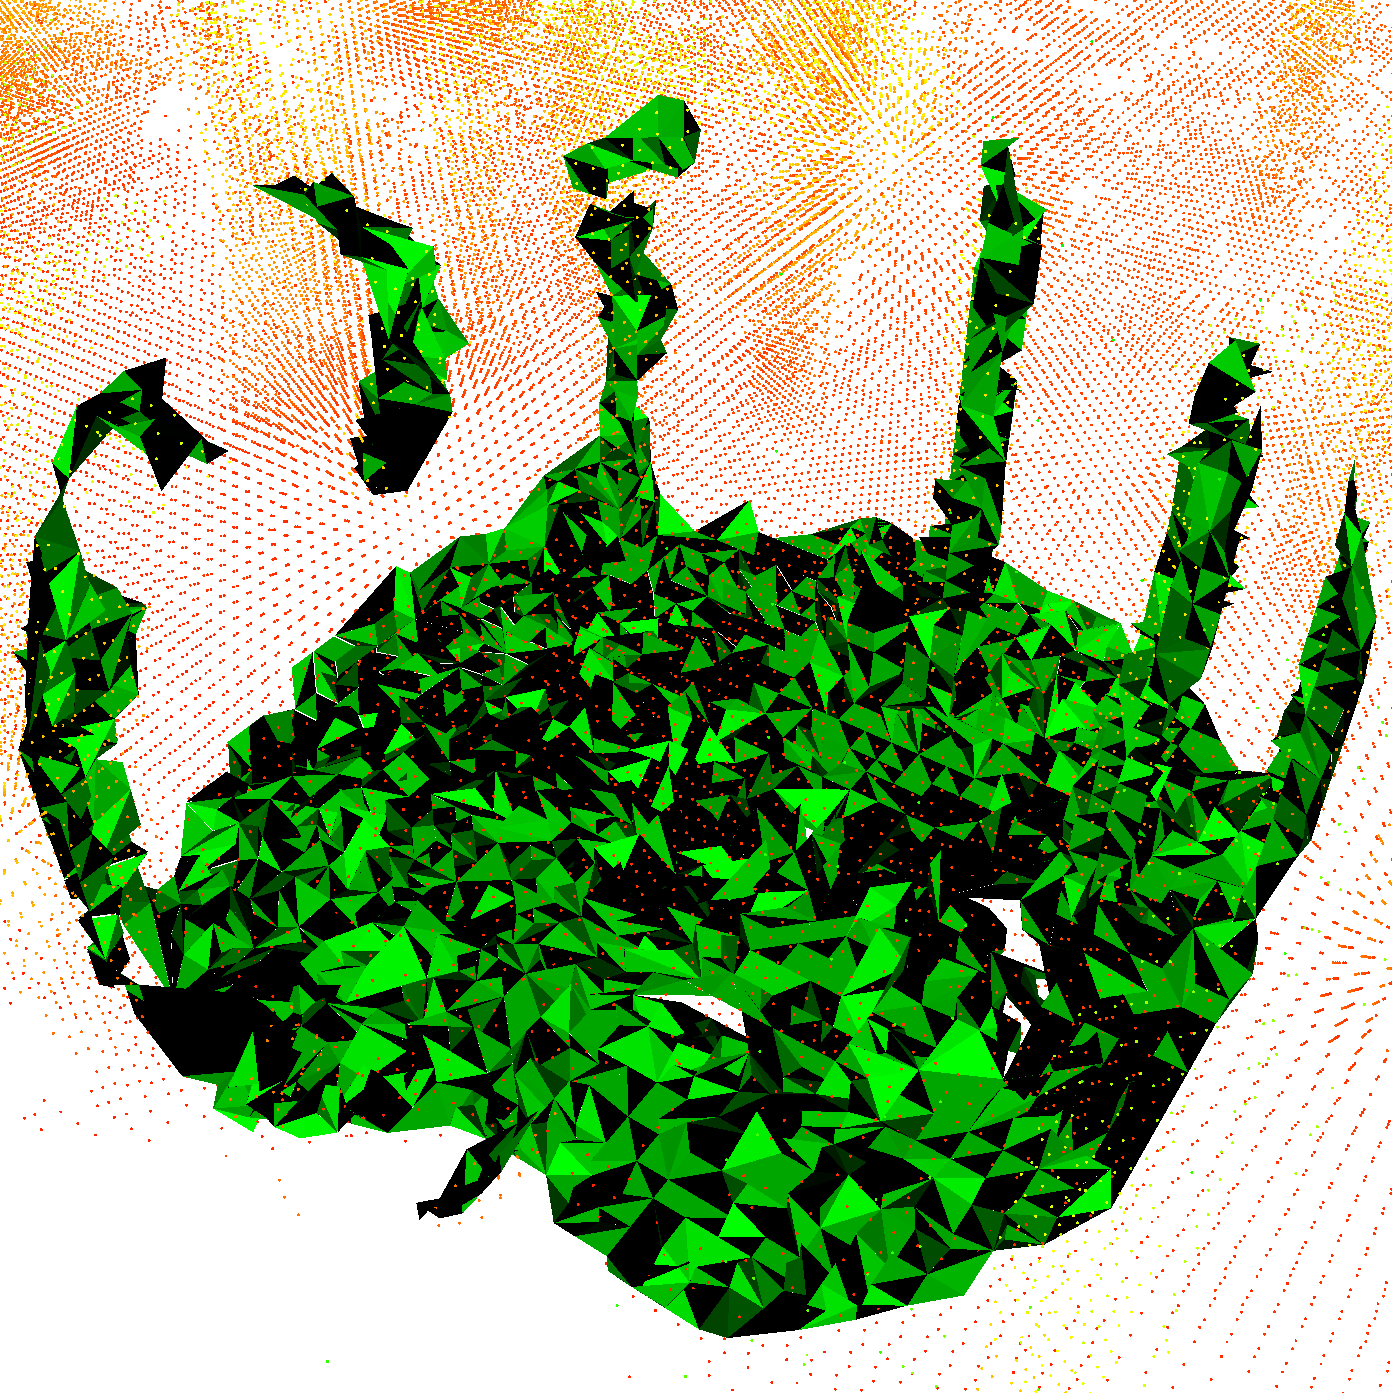
\includegraphics[width=0.48\textwidth]{./fig/rviz/triangulation_surface_aprox.png}
                \caption{
                    Surface approximation using Greedy Projection Triangulation.
                }
                \label{fig:triangulation}
            \end{figure}

        \subsection{Voxel-Based Modification of Cell $\mathcal{A}_i$}
            Given that the size of the voxels is known, this information can be used to refine the partitioning of cell $\mathcal{A}_i$ by treating voxels as obstacles.
            First, it is necessary to determine which voxels are relevant to the \ac{RBL} algorithm.
            This can be achieved by considering the scaling parameter $\eta$.
            A voxel is considered relevant if it lies within a radius of $\frac{r_s}{\eta}$ of the agent.
            For each discrete point in the cell $\mathcal{S}_i$, the nearest voxel is identified using a k-d tree algorithm from the \ac{PCL} library \cite{kd_tree}.
            Because the found point is the voxel's center, the closest point within that voxel's boundaries is calculated to accurately partition the cell $\mathcal{A}$ from cell $\mathcal{S}$.

            Given a point $\mathbf{p_{\mathcal{S}}}$, the voxel center $\mathbf{v_c}$ and the voxel edge length $\mathbf{e}$, $\mathbf{p}_{\text{closest}}$ is computed as: 
            \begin{equation}
                \mathbf{p}_{\text{closest}} =
                \begin{pmatrix}
                    \text{f}(p_{\mathcal{S},x}, v_{c,x} - \frac{\mathbf{e}}{2}, v_{c,x} + \frac{\mathbf{e}}{2}) \\
                    \text{f}(p_{\mathcal{S},y}, v_{c,y} - \frac{\mathbf{e}}{2}, v_{c,y} + \frac{\mathbf{e}}{2}) \\
                    \text{f}(p_{\mathcal{S},z}, v_{c,z} - \frac{\mathbf{e}}{2}, v_{c,z} + \frac{\mathbf{e}}{2})
                \end{pmatrix}\text{,}
            \end{equation}
            where the function f(x, a, b) constrains the value x to the range [a, b].
            This constrains $\mathbf{p_{\mathcal{S}_i}}$ to the voxel boundaries.
            
            Considering the point $\mathbf{p}_{\text{closest}}$ as an obstacle, the sensing cell $\mathcal{S}_i$ is partitioned to form cell $\mathcal{A}_i$ using the same procedure as \refeq{eqn:voronoi_cell_account_encum} (considering the closest point as another agent) encumbrance of the obstacle is not needed, because the closest point has been already found.
            The sensing cell $\mathcal{S}$ is partitioned to form the operational cell $\mathcal{A}$ by treating $\mathbf{p}_{\text{closest}}$ (the nearest point on an obstacle) as an agent and applying the procedure from Equation \eqref{eqn:voronoi_cell_account_encum}, the obstacle's full encumbrance is not required for this step because $\mathbf{p}_{\text{closest}} = \tilde{\mathbf{p}}_{j}$ provides the relevant point for partitioning $\mathcal{A}_i$, therefore $\delta_j = 0$.
            % This partition involves excluding any point $\mathbf{p_{\mathcal{S}}}$ from  $\mathcal{S}$ if its position relative to the agent $\mathbf{p}_i$ and the obstacle point $\mathbf{p}_{\text{closest}}$ meet condition $\mathcal{A}$ if $ \| \mathbf{p_i} - \mathbf{p_{\mathcal{S}}} \| \leq \eta \cdot \| \mathbf{p_i} - \mathbf{p}_{closest}\|$.

            % Using this point we can consider him as an obstacle and partition him out of sensing cell to form cell A. 
            % A point $\mathbf{p_{\mathcal{S}}}$ is excluded from the cell $\mathcal{A}$ if $ \| \mathbf{p_i} - \mathbf{p_{\mathcal{S}}} \| \leq \eta \cdot \| \mathbf{p_i} - \mathbf{p}_{closest}\|$.
            

    \section{Implementation and Integration on UAV}
    \label{sec:implementation_integration}
        \subsection{Challenges in Integration}
            The algorithm's performance is influenced by the limitations of the \ac{LiDAR} sensor used for environmental sensing. 
            While the algorithm works optimally with a full 360° horizontal and 180° vertical \ac{FOV}, which would require multiple sensors, the experiments used a single Livox Mid 360 \ac{LiDAR} \cite{livox_mid360}. 
            This \ac{LiDAR} provides a 360° horizontal \ac{FOV} and only a 59° vertical \ac{FOV}, resulting in a sensing blind spot.

            To solve this limitation, several modifications were implemented. 
            The \ac{LiDAR} was mounted at an angle $\gamma$, as shown in Figure \reffig{fig:uavs}, to enhance ground sensing and increase forward visibility.

            \begin{figure}[htbp]
                \centering
                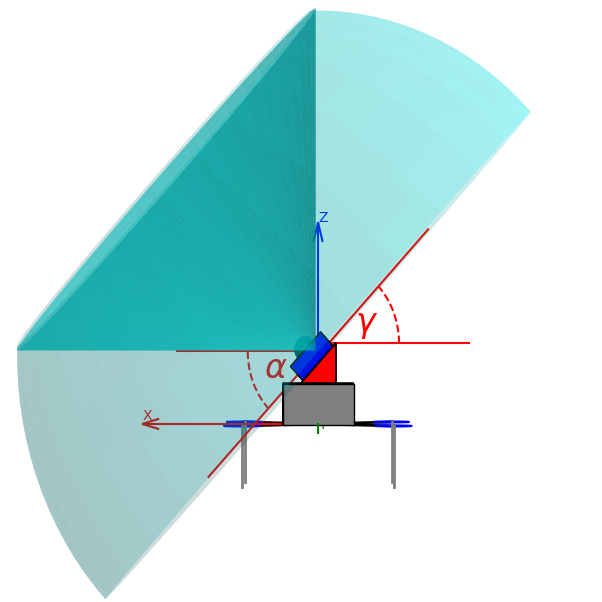
\includegraphics[width=0.48\textwidth]{./fig/photos/uav_side_view.png}
                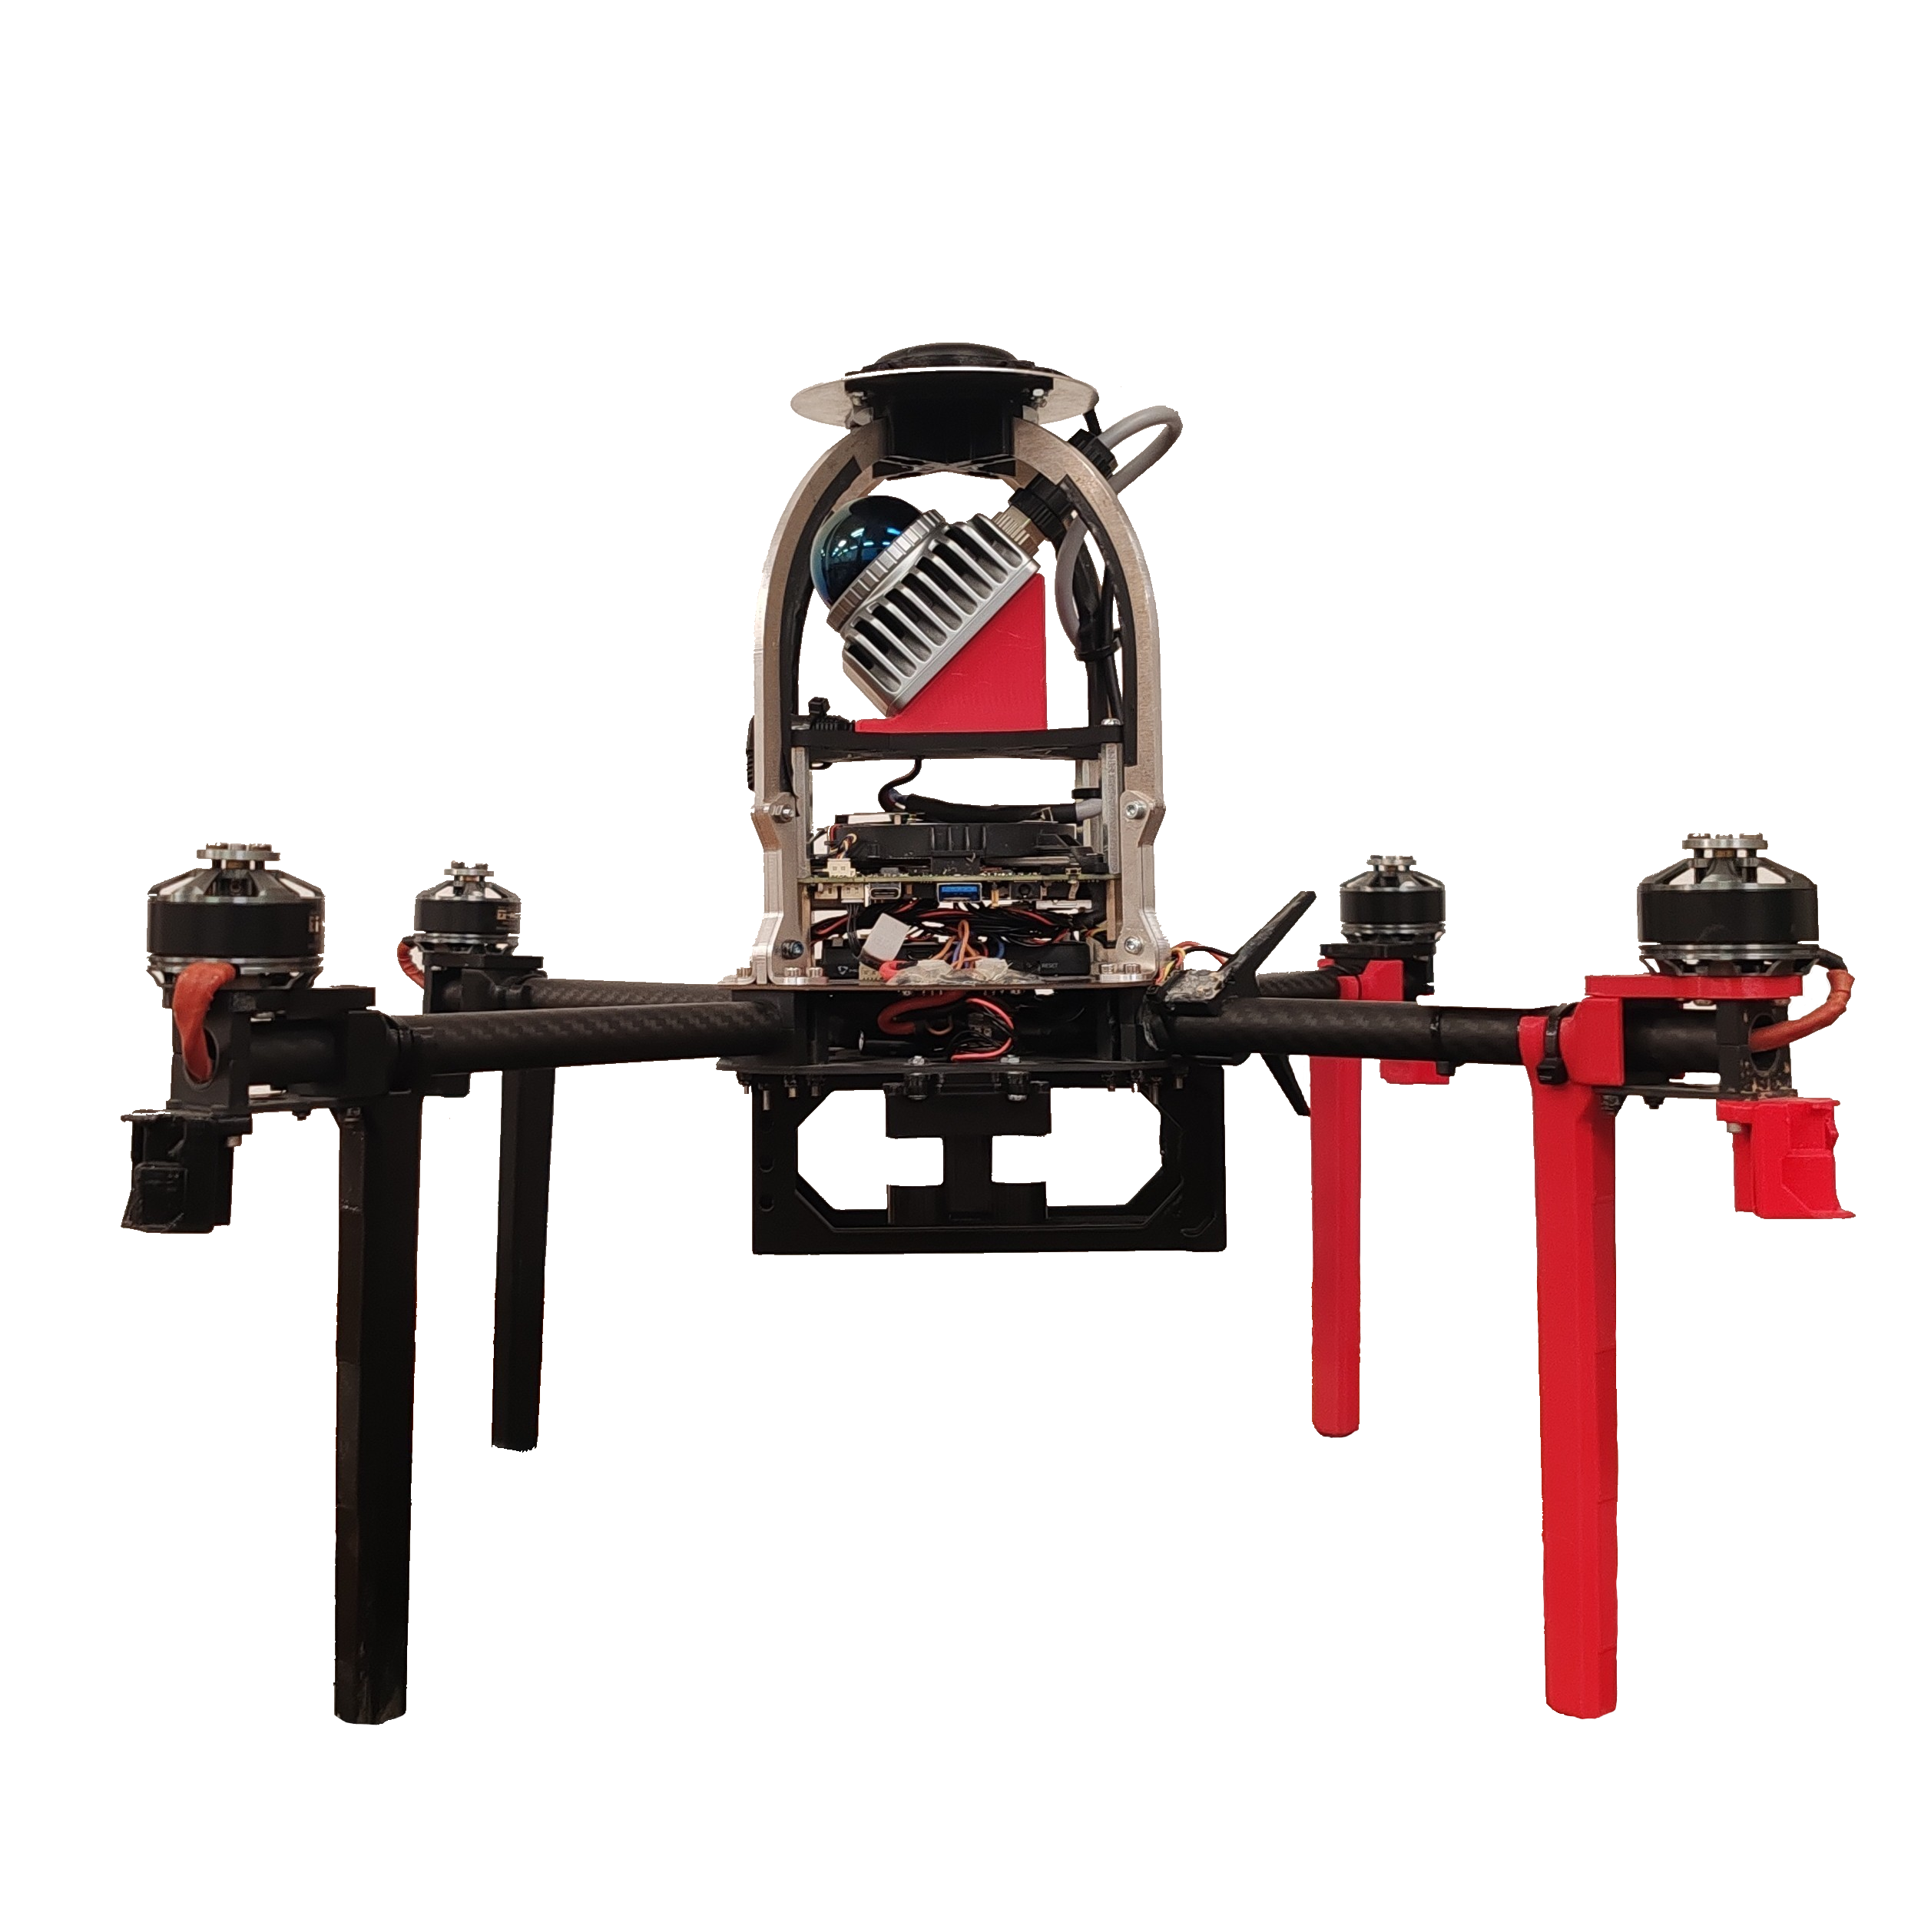
\includegraphics[width=0.48\textwidth]{./fig/photos/uav_photo.png}
                \caption{
                    \ac{UAV} and \ac{LiDAR} mounting scheme.
                    Please note that a different mounting angle was used in practical experiments, so the configuration shown here is purely for visualization purposes.
                    Subfigure on the left shows a modeled \ac{UAV} with visualized \ac{LiDAR} mounting parameters, including the \ac{LiDAR} elevation field of view $\alpha$ and tilt angle $\gamma$. 
                    Subfigure on the right displays the real \ac{UAV} used in the experiment with the \ac{LiDAR} mounted according to the same configuration.                                                
                }
                \label{fig:uavs}
            \end{figure}

            In addition to the \ac{LiDAR} mounting angle, a software modification is implemented to account for the \ac{LiDAR}'s limited \ac{FOV}.
            The algorithm uses the map to partition cell $\mathcal{S}_i$ into cell $\mathcal{A}_i$, from which the centroid is computed to guide \ac{UAV} movement.
            To ensure safety, the \ac{UAV} should only move within its visible \ac{FOV}. 
            However, the map information from areas outside the current \ac{FOV} can still be valuable. 

            Therefore, the following constraint is introduced - the \ac{UAV} maintains its yaw rotation towards the current centroid $\mathbf{c}_{\mathcal{A}}$ and moves towards the centroid only when the centroid is positioned within a $\pm \frac{\pi}{4}$ rad angular range from the direction the \ac{LiDAR} is tilted towards (the \ac{UAV}'s x-axis).
            This $\frac{\pi}{2}$ rad forward sector for movement is determined by the \ac{UAV}'s physical structure, specifically to prevent the \ac{UAV} from moving into areas where mounting rods for \ac{GPS} obstruct active sensing.

            To integrate the \ac{LiDAR}'s \ac{FOV} into cell $\mathcal{S}_i$, two planes are defined based on the \ac{LiDAR}'s mounting configuration and vertical \ac{FOV}.
            Let $\mathbf{e}_z$ be a unit vector along the z-axis, $R_{\gamma} \in SO(3)$ the tilt of the \ac{LiDAR}, and $R_{rpy} \in SO(3)$ the roll-pitch-yaw rotation.
            The normal vectors, $\mathbf{n}_1$ and $\mathbf{n}_2$ defining two planes are given by:
            \begin{equation}
                \mathbf{n}_1 = R_{rpy} R_{y}(\gamma)  \mathbf{e}_z    
            \end{equation}
            \begin{equation}
                \mathbf{n}_2 = R_{rpy} R_{y}(\gamma - \alpha) \mathbf{e}_z  \text{,}
            \end{equation}
            where $\alpha$ is the \ac{LiDAR}'s \ac{FOV} and $\gamma$ is the mounting angle of the \ac{LiDAR}, and $R_{rpy} = R_x(\text{roll})R_y(\text{pitch})R_z(\text{yaw})$.
            Cell $\mathcal{S}_i$ is then modified by excluding points that lie outside the \ac{LiDAR}'s \ac{FOV}, defined by these two planes: 

            \begin{equation}
                \mathcal{S}_i' = \{ \mathbf{q} \in \mathcal{S}_i \mid \mathbf{n}_1 \cdot (\mathbf{q} - \mathbf{p}_{L}) \geq 0 \land \mathbf{n}_2 \cdot (\mathbf{q} - \mathbf{p}_{L}) \leq 0 \}\text{,}
            \end{equation}
            where $\mathcal{S}_i'$ is the modified cell $\mathcal{S}_i$ and $\mathbf{p}_{L}$ is the exact position of the LiDAR sensor.

            This modification effectively restricts the points considered in the calculation of the centroid to only those within the \ac{LiDAR}'s \ac{FOV}.

            To integrate map information from the surrounding area outside of the \ac{LiDAR}'s current \ac{FOV}, the following procedure is used.
            Firstly, both cells $\mathcal{S}_i$ and $\mathcal{S}_i'$ are created. These cells are partitioned into cells $\mathcal{A}_i$ and $\mathcal{A}_i'$ using voxels. 
            Cell $\mathcal{A}_i'$ is partitioned using voxels that are actively sensed, while cell $\mathcal{A}_i$ is partitioned using the voxels from the whole surroundings.

            If the centroid computed from cell $\mathcal{A}_i$, $\mathbf{c}_{\mathcal{A}_i}$, is within the cell $\mathcal{A}_i'$, the \ac{UAV} is commanded to move towards $\mathbf{c}_{\mathcal{A}_i}$ while simultaneously rotating its yaw towards it.
            However, if $\mathbf{c}_{\mathcal{A}_i}$ lies outside cell $\mathcal{A}_i'$, it is projected onto the closest point on the boundary of cell $\mathcal{A}_i'$.
            As the \ac{UAV} only moves if the centroid is within a certain angle in front of it, this projection onto the boundary of $\mathcal{A}_i'$ ensures that the \ac{UAV} primarily rotates towards the centroid until the centroid is within an angle in front of the \ac{UAV}.
            This control logic is formally defined as follows:
            \begin{equation}
                \begin{cases}
                    \text{move and rotate towards } \mathbf{c}_{\mathcal{A}_i} & \text{if } \mathbf{c}_{\mathcal{A}_i} \in \mathcal{A}_i' \land \alpha \in [-\frac{\pi}{4}, \frac{\pi}{4}] \\
                    \text{only rotate, do not move towards } \mathbf{c}_{\mathcal{A}_i} & \text{otherwise, }
                \end{cases}
            \end{equation}
            where $\alpha = \text{atan2}((\mathbf{c}_{\mathcal{A}_i} - \mathbf{p}_i)_y, (\mathbf{c}_{\mathcal{A}_i} - \mathbf{p}_i)_x) - \text{yaw}_i$

            This procedure effectively utilizes the information from the map while ensuring that the \ac{UAV} moves only within its actively sensed \ac{FOV}.

            \begin{figure}[H]
                \centering
                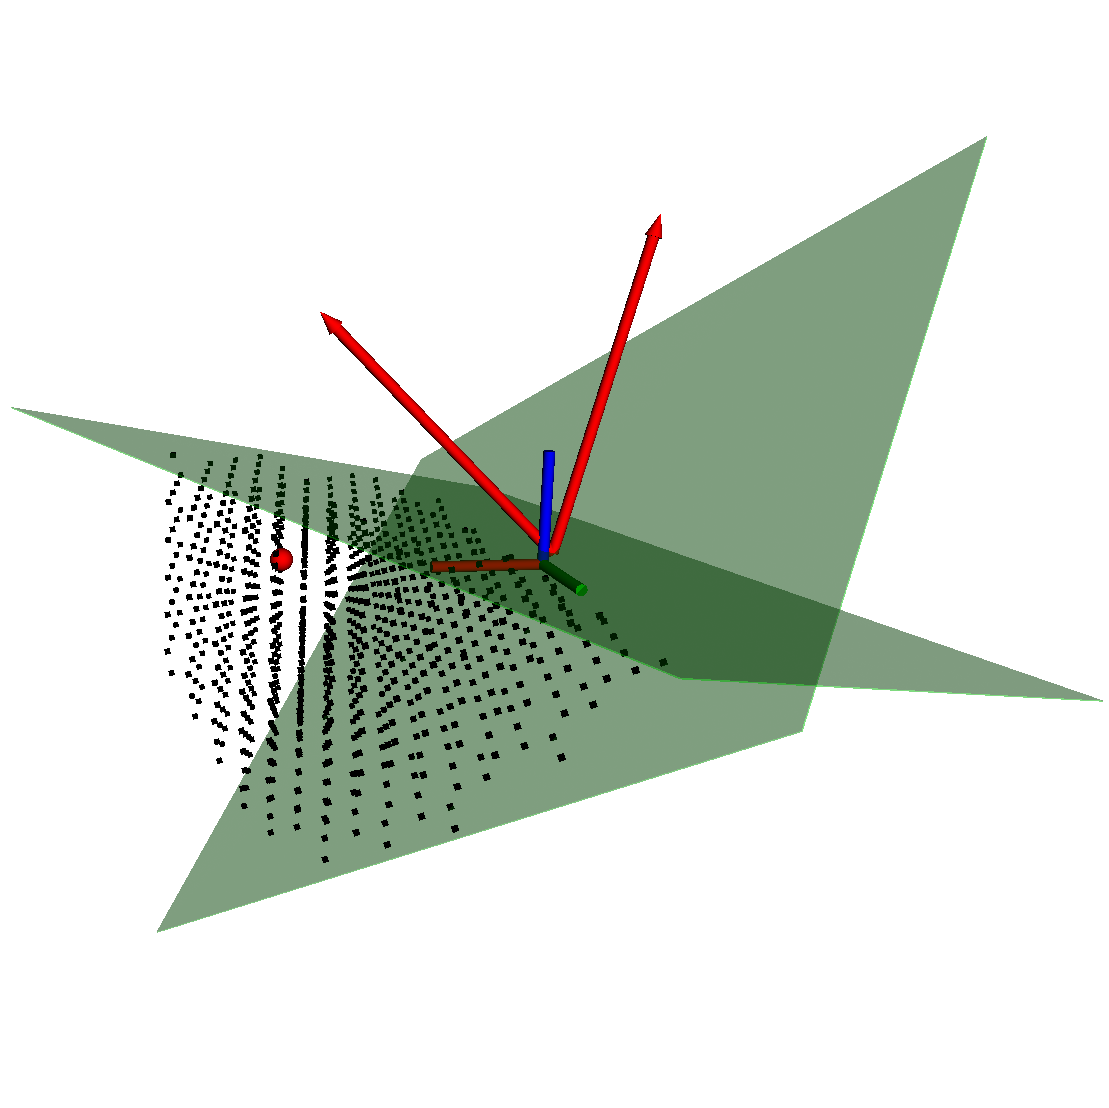
\includegraphics[width=0.48\textwidth]{./fig/rviz/cell_a_sliced_with_planes.png}
                \caption{
                    Rviz visualization of \ac{LiDAR} \ac{FOV} planes. The \ac{UAV} is represented by the XYZ coordinate axes. 
                    The green squares represent the two planes, defined by normal vectors $\mathbf{n}_1$ and $\mathbf{n}_2$, used to slice cell $\mathcal{S}_i$ and determine the modified cell $\mathcal{S}_i'$.
                    The red sphere represents the centroid $\mathbf{c}_{\mathcal{A}_i}$.
                }
                \label{fig:cell_a_sliced}
            \end{figure}
    
    \section{Experimental Results}
    \label{sec:experimental_results}
        This section presents the findings from both simulated and real-world experiments conducted to evaluate the proposed approach.
        \subsection{Simulation Setup}
            In the simulations, a virtual forest environment was created. 
            Initially, a raycasting approach from the \ac{UAV} to the simulated trees was considered for obstacle detection. 
            However, due to its computational cost, a static point cloud representation of the entire forest was generated and published instead. 
            The forest was modeled as a collection of trees, with trunks represented by cylinders and crowns by spheres.
            The forest was generated within a rectangular area defined by the opposing corner points (-20.0 m, -32.0 m) and (20.0 m, 32.0 m) in the x-y plane, with its sides aligned parallel to the x and y axes.
            % The forest was contained within a rectangular area defined by the following boundaries:
            % \begin{itemize}
            %     \item $x_{\min}$ = -20.0 m
            %     \item $x_{\max}$ =  20.0 m
            %     \item $y_{\min}$ = -32.0 m
            %     \item $y_{\max}$ =  32.0 m
            % \end{itemize}
            A total of 100 trees were randomly generated within this area, with a minimum separation distance of 3 meters between them. 
            The trees were generated with the following parameter variances:
            \begin{itemize}
                \item Trunk radius: 0.5 $\pm$ 0.2 m
                \item Tree height: 7.5 $\pm$ 2.0 m
                \item Crown radius: 2.5 $\pm$ 0.5 m
            \end{itemize}
            The \ac{UAV}'s starting position was set at one corner of the rectangular area (-22.0, -33.0, 2.0), and the goal position was set at the opposite corner (22.0, 33.0, 5.0).

            Note that the right-hand rule and z rule, described in the previous chapter, are not required for effective coordination in this static forest environment.
            Also, the \ac{Point-LIO} estimator and Bonxai mapping were not simulated.

            A separate simulation was also run to compare the 2D \ac{RBL} algorithm with its 3D extension, using a circle crossing setup in the forest.

            The specific values of the parameters used in the experiments are summarized in the following table \ref{tab:rbl_forest_simulation_parameters}:

            % \begin{table}[H]
            %     \centering
            %     \caption{Parameters Used in Experiments}
            %     \begin{tabular}{|l|l|l|l|l|l|l|l|}
            %         \hline
            %         % Row 1: Parameter names act as column headers here
            %         Parameter & $r_s$ [m]                  & Update rate [Hz] & $\delta_i$ [m]  & $d_1 = d_3 = d_5$  [m] & $d_2 = d_4 = d_6$ [m] & $\beta_i^D$ [] & $\eta$ []\\
            %         \hline \hline 
            %         Value     & 3.5                        & 10               & 0.5             & 0.5                    & 1.0                   & 0.5            & 0.9  \\
            %         \hline
            %     \end{tabular}
            %     \label{tab:rbl_forest_simulation_parameters_transposed} % Adjusted label
            % \end{table}

            % \begin{table}[H]
            %     \centering
            %     \caption{Parameters Used in Experiments}
            %     \begin{tabular}{|l|c|}
            %         \hline
            %         Parameter & Value \\
            %         \hline
            %         \hline
            %         Sensing radius $r_s$ [m] & 3.5 \\ \hline
            %         Update rate [Hz] & 10  \\ \hline
            %         Encumbrance $\delta_i$ [m] & 0.5  \\ \hline
            %         $d_1 = d_3 = d_5$ [m] & 0.5  \\ \hline
            %         $d_2 = d_4 = d_6$ [m] & 1.0  \\ \hline
            %         $\beta_i^D$ [ ] & 0.5  \\ \hline
            %         $\eta$ [ ] & 0.9  \\ \hline
            %     \end{tabular}
            %     \label{tab:rbl_forest_simulation_parameters}
            % \end{table}

            \begin{table}[H]
                \centering
                \caption{Parameters Used in Experiments}
                
                \begin{tabular}{|c|c|c|c|c|}
                    \hline
                    Parameter & $r_s$ [m]  & $\delta_i$ [m] & $d_1 = d_3 = d_5$ [m] & $d_2 = d_4 = d_6$ [m]   \\ \hline
                    Value & 3.5 & 0.5 & 0.5 & 1.0 \\ \hline
                \end{tabular}
                
                \vspace{0.3cm}
                
                \begin{tabular}{|c|c|c|c|c|}
                    \hline
                    Parameter & Update rate [Hz] & $\gamma$ [°] & $\beta_i^D$ [ ] & $\eta$ [ ] \\ \hline
                    Value & 10.0 & 20.0 & 0.5 & 0.9 \\ \hline
                \end{tabular}
                
                \label{tab:rbl_forest_simulation_parameters}
            \end{table}
            
            The \ac{UAV} dynamics are the same as described in the previous chapter and detailed in Table \ref{tab:uav_constraints}. 
            Each simulation was run 10 times with the same forest. 

        \subsection{Performance in Simulated Environments}
            The first simulation results highlight the proposed solution capability in navigating inside dense forest environments. 
            The \ac{UAV} demonstrated effective obstacle avoidance, reacting appropriately to simulated trees while maintaining an efficient trajectory without unnecessary detours.
            Convergence towards the designated goal was consistently achieved in a stable manner.

            \begin{table}[H]
                \centering
                \renewcommand{\arraystretch}{1.2}
                \begin{tabular}{|c|c|c|c|c|}
                \hline
                                                  & \( SR \ [\%] \) & \( \overline{L} \ [\mathrm{m}] \) & \( \overline{t} \ [\mathrm{s}] \) &  \( \overline{v} \ [\mathrm{m/s}] \)     \\ \hline
                Results                           & 100.00          & 91.99 $\pm$ 0.96                  & 150.89 $\pm$ 0.88                  &  0.85 $\pm$ 0.00                         \\ \hline
                \end{tabular}
            \end{table}

            \begin{figure}[H]
                \centering
                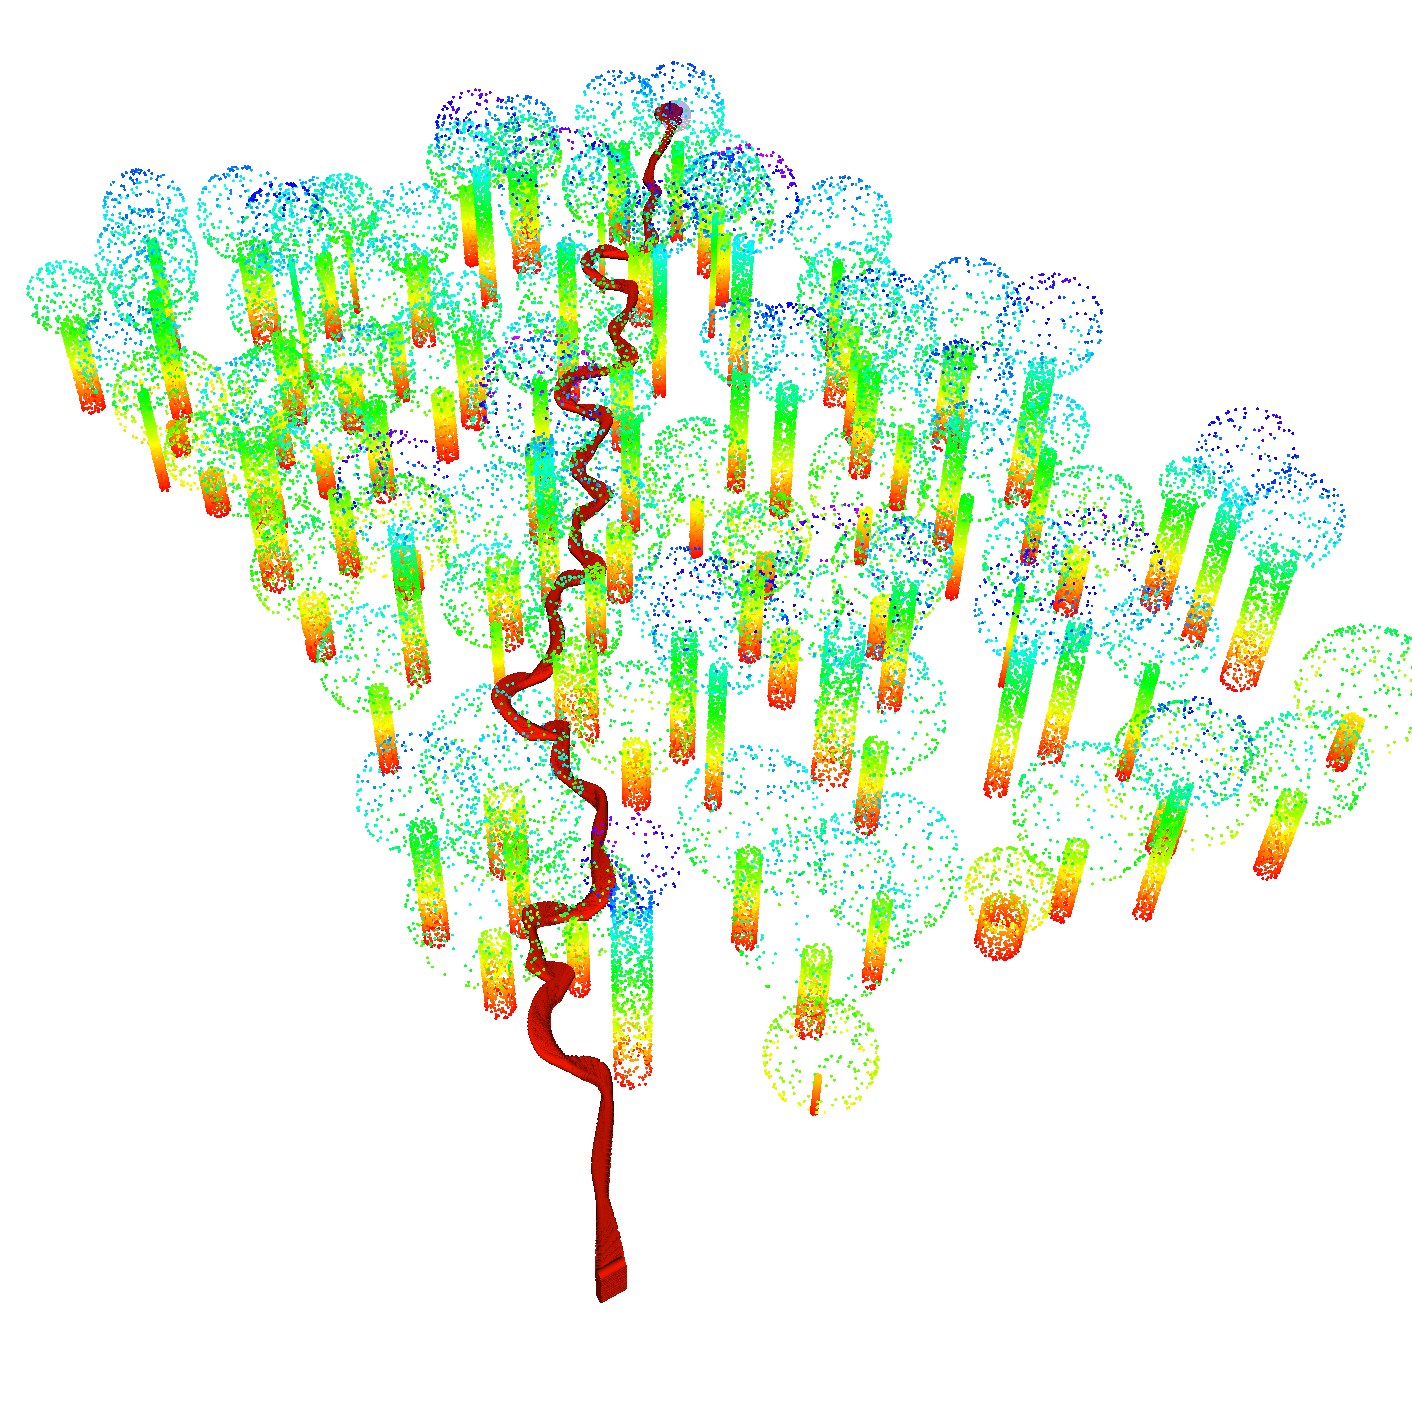
\includegraphics[width=0.48\textwidth]{./fig/rviz/simulation_forest.png}
                \caption{
                    Visualization of simulated forest and the corresponding path of the \ac{UAV}, indicated by a red line.
                }
                \label{fig:simulated_forest_path}
            \end{figure}

            Additional simulations directly compared the 2D and extended 3D \ac{RBL} algorithms in the static forest. 
            These results confirmed that \ac{UAV}s using the 3D \ac{RBL} were capable of consistently reaching the goal by exploring vertical dimensions, navigating above or below tree crowns. 
            The 2D \ac{RBL}, on the other hand, failed by getting stuck between the obstacles.
            \begin{table}[H]
                \centering
                \renewcommand{\arraystretch}{1.2}
                \begin{tabular}{|c|c|c|c|c|c|}
                \hline
                                                    & \( SR \ [\%] \)   & \( \overline{L} \ [\mathrm{m}] \)                & \( \overline{t} \ [\mathrm{s}] \)                & \( \overline{t}_{\text{max}} \ [\mathrm{s}] \)    &   \( \overline{v} \ [\mathrm{m/s}] \)     \\ \hline
                \ac{RBL} 2D                         & 0.00              & 30.27 $\pm$ 0.12                                 & $\infty$                                         &  $\infty$                                         &  0.00 $\pm$ 0.00                         \\ \hline
                \ac{RBL} $\text{3D}_{\text{rule}}$  & $\mathbf{100.00}$ & $\mathbf{28.40} \boldsymbol{\pm} \mathbf{10.68}$ & $\mathbf{50.90} \boldsymbol{\pm} \mathbf{33.51}$ &  $\mathbf{99.86} \boldsymbol{\pm} \mathbf{16.01}$ &  $\mathbf{0.54} \boldsymbol{\pm} \mathbf{0.27}$                         \\ \hline
                \end{tabular}
            \end{table}

            \begin{figure}[htbp]
                \centering
                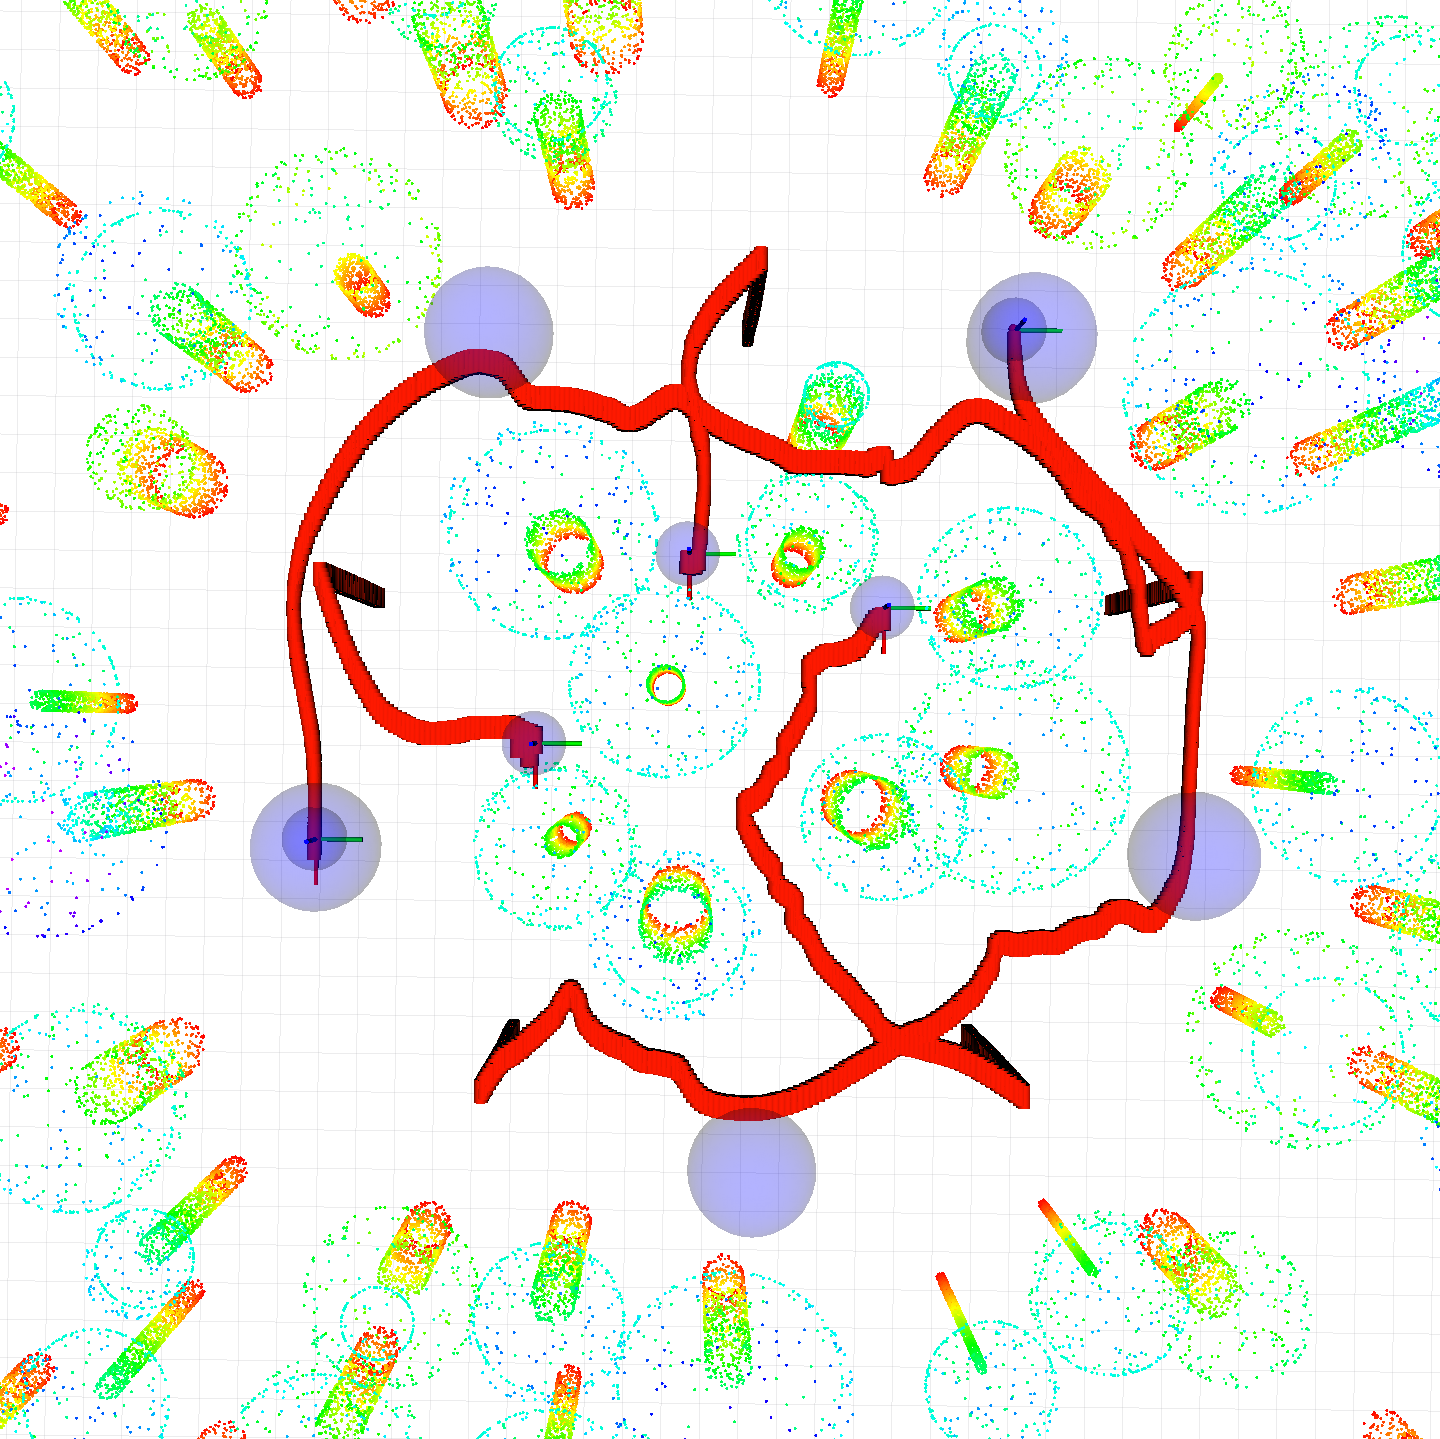
\includegraphics[width=0.48\textwidth]{./fig/rviz/circular_forest_fail.png}
                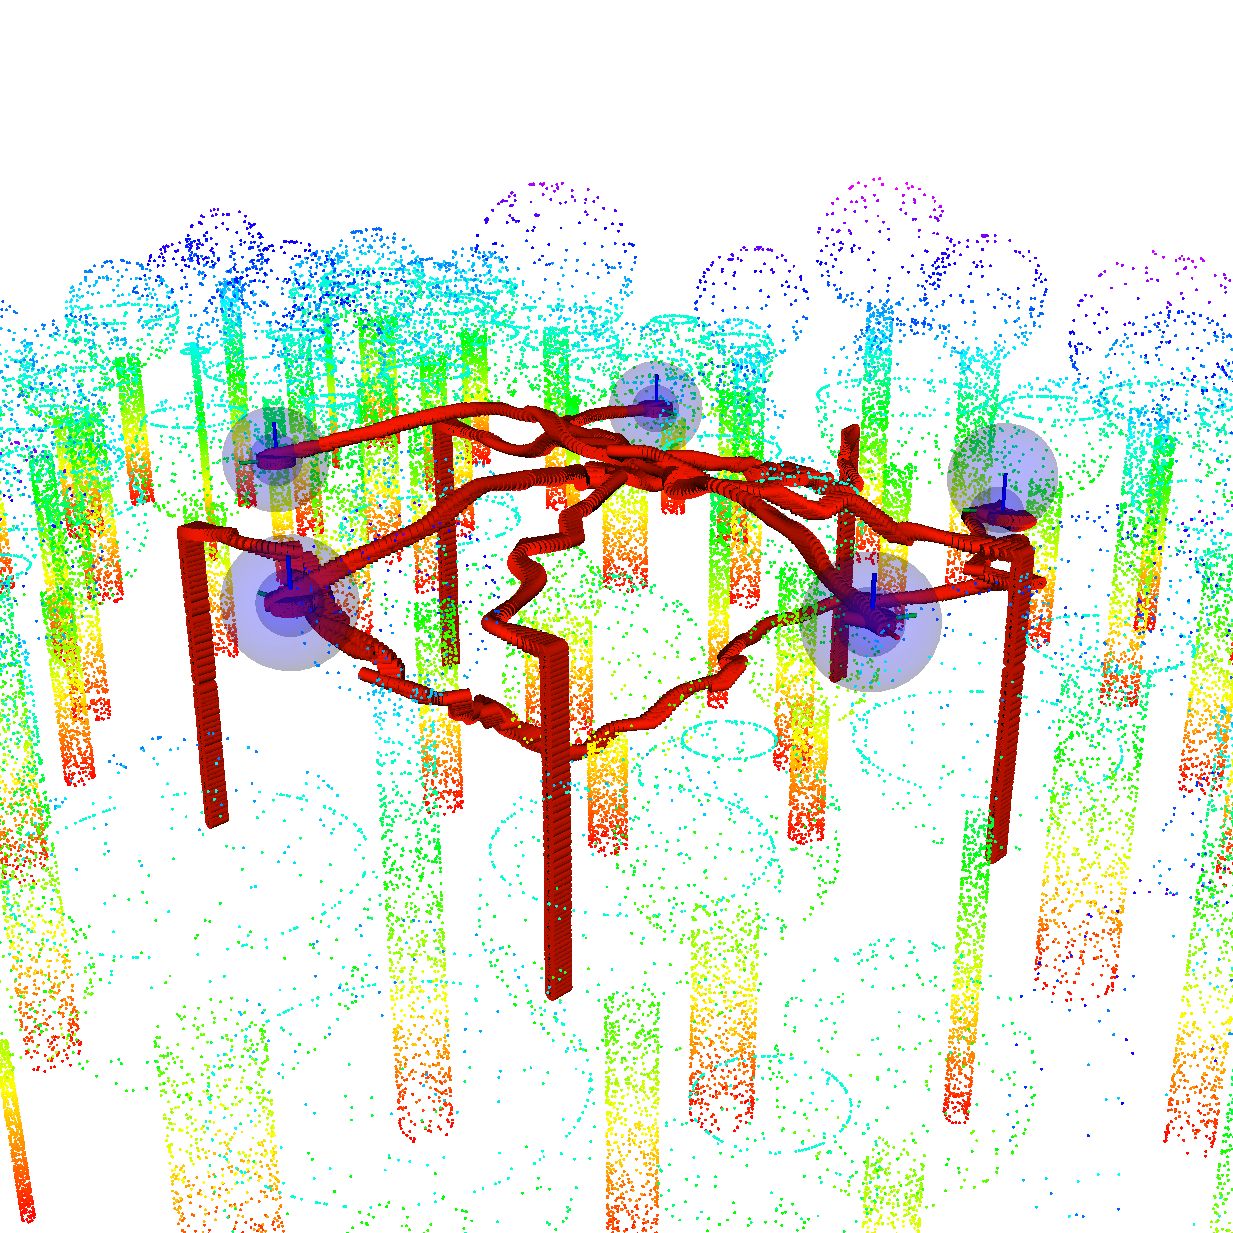
\includegraphics[width=0.48\textwidth]{./fig/rviz/3d_crossing_circle_forest.png}
                \caption{
                    Illustrative comparison of 2D and 3D RBL navigation capabilities in a simulated forest environment. 
                    Left: The 2D algorithm is shown in a deadlock. 
                    Right: The 3D algorithm demonstrates its ability to utilize vertical space.
                }
                \label{fig:forest_crossing_circle}
            \end{figure}

        \subsection{Real-World Experiments in a Forest Environment}
            Following the successful simulation validation, the \ac{RBL} algorithm was tested through real-world experiments conducted in a forest environment.
            \begin{itemize}
                \item \textbf{Location: } \\
                    The forest site for initial real-world experiments was chosen for its relatively open characteristics, allowing for straightforward system validation. 
                    Subsequent flight tests were then conducted in more challenging and densely obstructed environments.
                    To increase the navigational challenge and better test the obstacle avoidance capabilities, additional branches were placed near trees within the flight area after a few successful flights. 
                    % The point cloud filtration parameters were set to discard points closer than 1.0 meter (to avoid detecting the \ac{UAV}'s own propellers) and farther than 40 meters.
                \item \textbf{UAV Platform: } \\
                    % A custom-built multirotor \ac{UAV} from the MRS group was used for this experiment X500. 
                    A custom-built multirotor \ac{UAV} from the \ac{MRS} group, the X500, was used for these experiments.
                    It was equipped with \ac{LiDAR} mounted on top for environmental perception and state estimation.
                    While other sensors like \ac{GPS} (unreliable in the forest), a Garmin altimeter, and barometer were present on the platform, they were not used.
                % \item \textbf{Experimental Procedure: } \\
                %     Each experimental run followed a defined procedure. 
                %     First, the necessary software components were launched within a tmux session on the ground. 
                %     A safety pilot then armed the \ac{UAV} and performed a manual takeoff to a safe altitude. 
                %     Once airborne and stable, the \ac{RBL} algorithm was initiated, commanding the \ac{UAV} towards a predefined goal. 
                %     The flight was continuously monitored via visualization in Rviz and observing the \ac{UAV}. 
                %     If the \ac{UAV} approached an obstacle too closely or exhibited unsafe behavior, the safety pilot immediately terminated the autonomous mode, took manual control, and landed the \ac{UAV}. 
                %     Between runs, key algorithm parameters, such as those controlling navigation 'aggressivity' (e.g., the scale of cells in the RBL and the weighting function used for path planning), were adjusted based on observations from the previous flight, and the experiment was repeated.
                % \item \textbf{Safety Measures: } \\
                %     Safety was paramount throughout the experiments. 
                %     A trained safety pilot maintained visual line-of-sight with the \ac{UAV} at all times and was prepared to immediately take manual control via the remote controller should any unsafe condition arise.
                % \item \textbf{Data Collected: } \\
                %     For safety reasons, data logging was initiated only after the manual takeoff was complete. 
                %     During the autonomous flight part and subsequent landing, all relevant ROS topics (including sensor data, estimated state, \ac{RBL} cells, centroid) were recorded into rosbag files for detailed post-flight analysis.
                % \item \textbf{Challenges Encountered: } \\
                %     Several challenges emerged during real-world deployment. 
                %     A significant set-back involved correctly managing coordinate frame transformations, particularly due to the slight tilt of the top-mounted LiDAR sensor. 
                %     Ensuring accurate alignment between the LiDAR's point cloud data, the \ac{Point-LIO} state estimator, and the navigation algorithm's reference frame required careful configuration. 
                %     Another challenge, which warrants further investigation (discussed in Future Work), related to the Bonxai mapping part. 
                %     Occasionally, the mapper would map dynamic objects, such as leaves disturbed by propellers, into the static map. 
                %     Due to the mapping algorithm's configuration, which was set to be conservative about removing potentially static obstacles to ensure safety, these incorrectly mapped 'ghost' obstacles were sometimes not removed even when subsequent scans showed they were no longer present. 
                %     In some instances, this led to the \ac{UAV} perceiving itself as surrounded by obstacles (effectively 'locking' itself), requiring the safety pilot to intervene and land.
            \end{itemize}

            \begin{figure}[htbp]
                \centering
                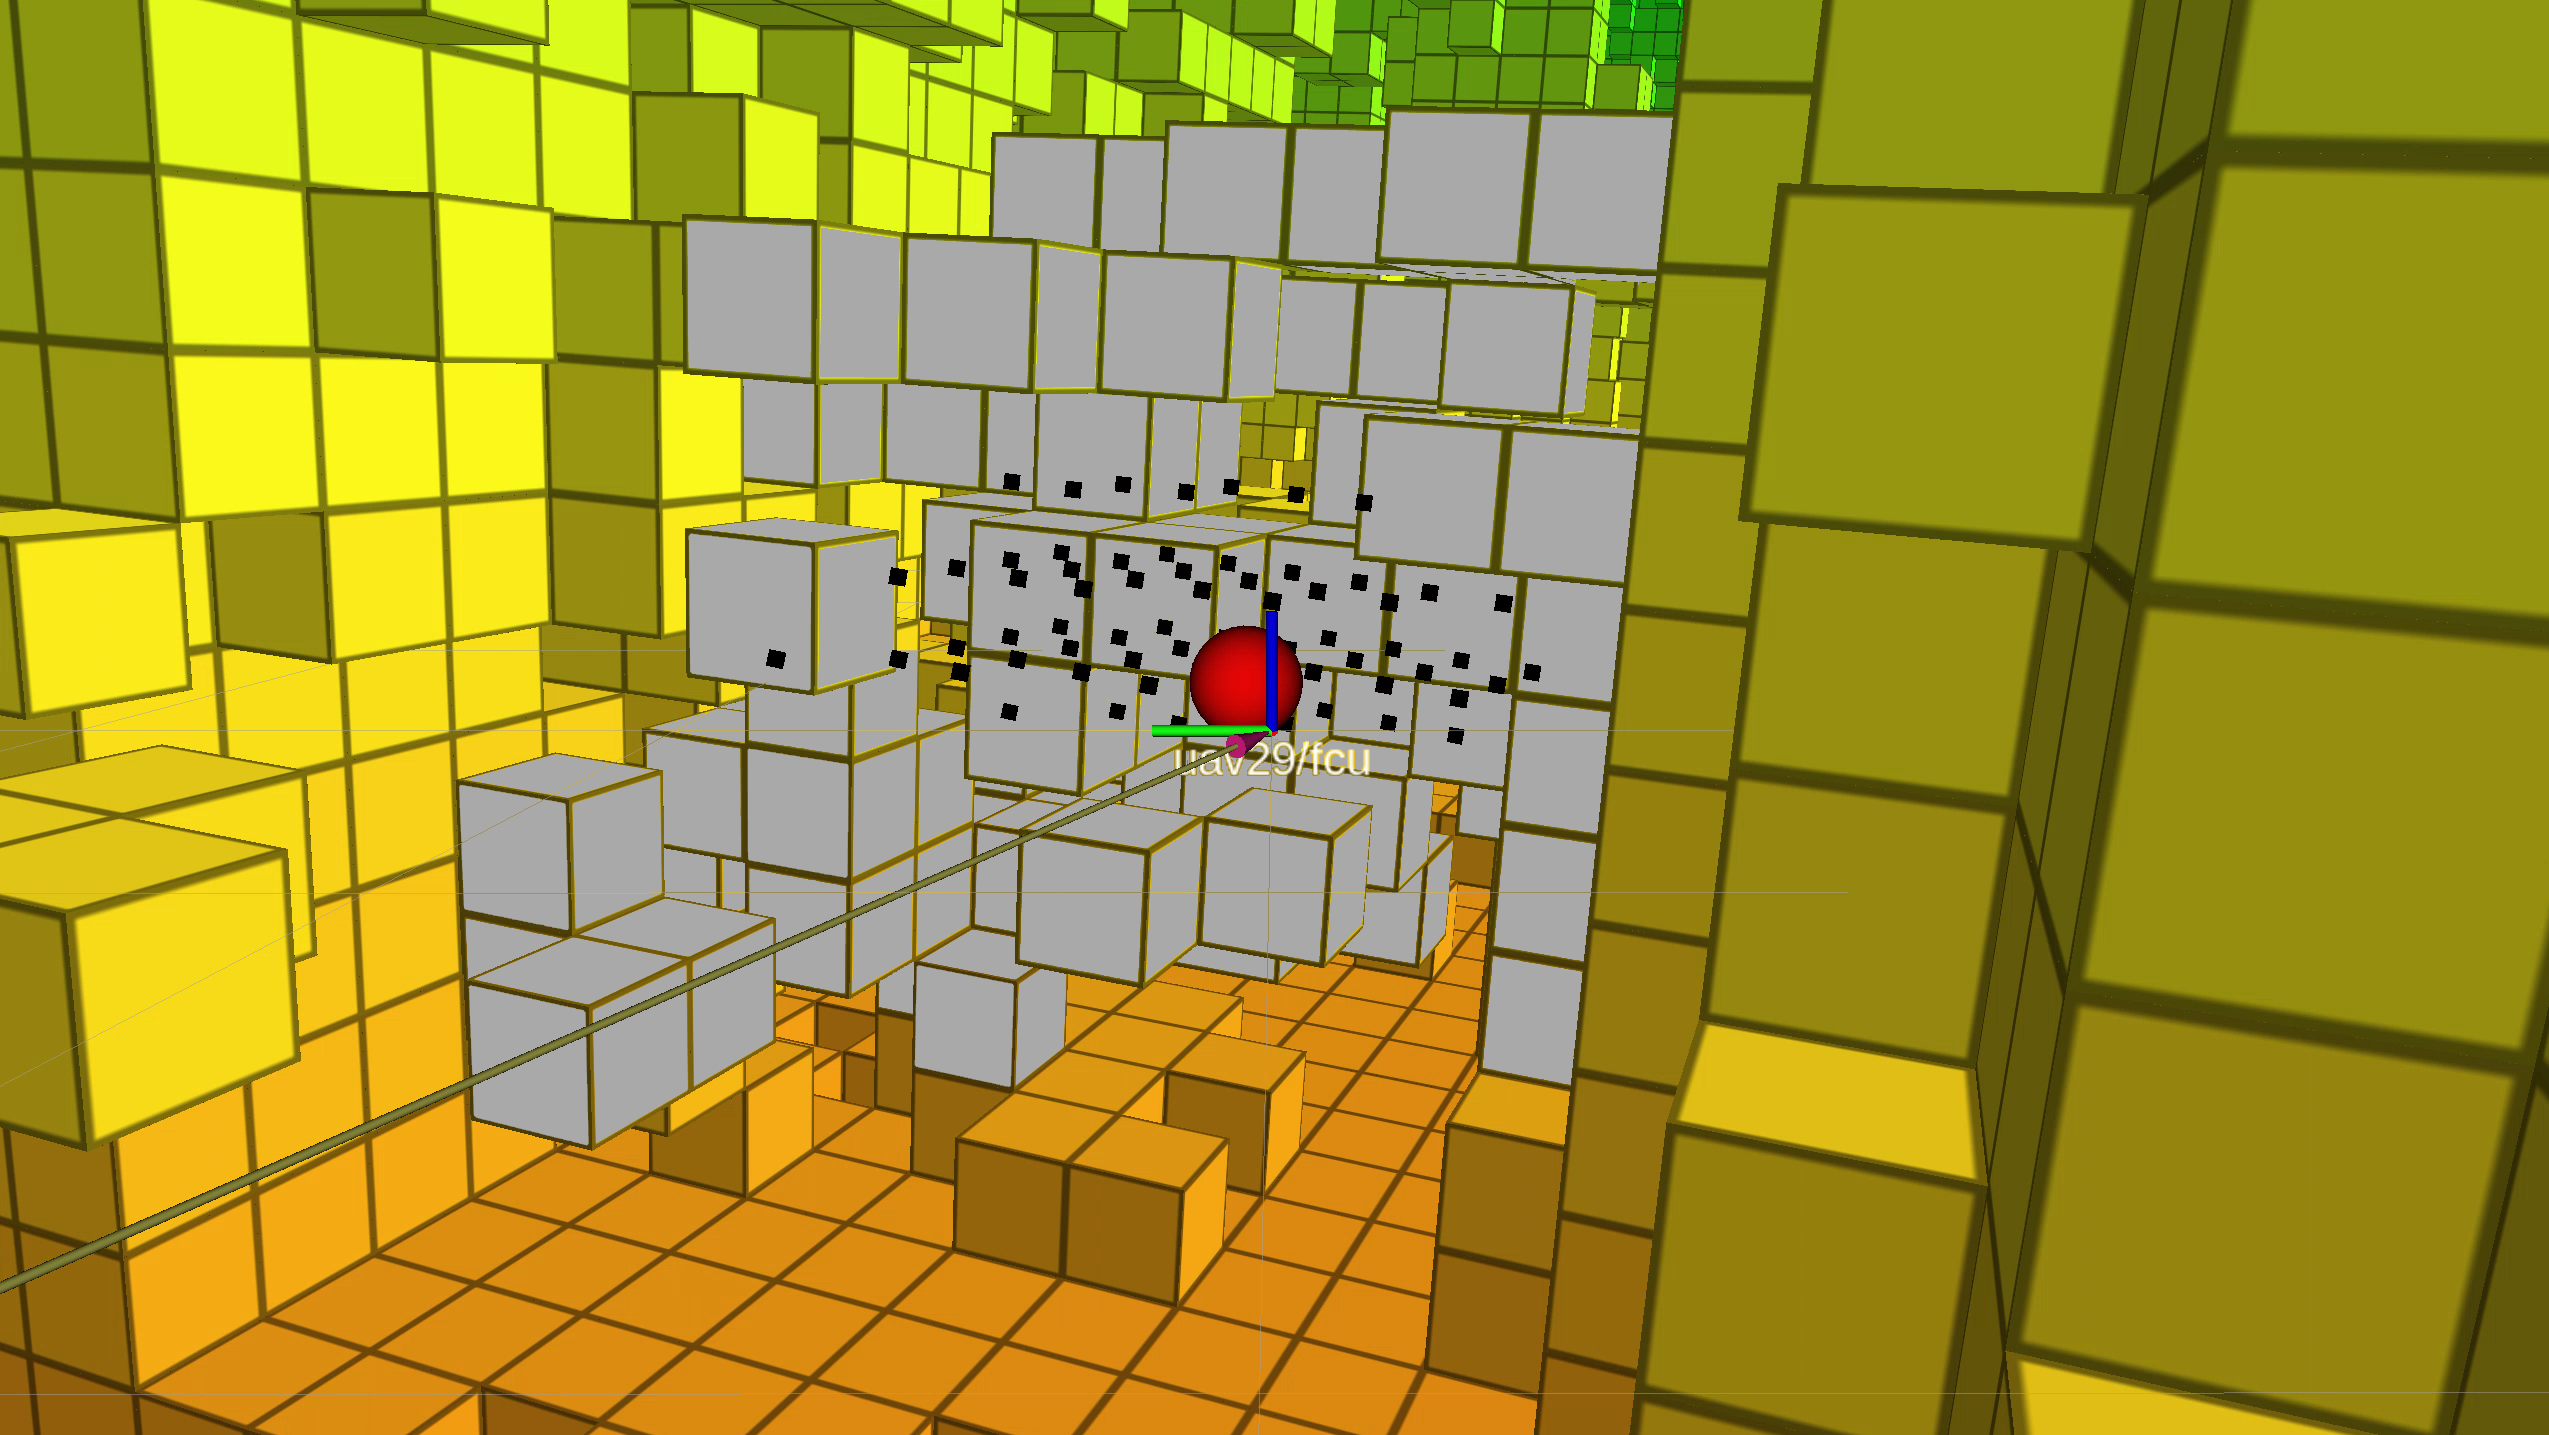
\includegraphics[width=0.96\textwidth]{./fig/rviz/deadlock_moment_mapping_gray.png}
                \caption{
                    Visualization of a moment where the \ac{UAV} incorrectly mapped leaves as obstacles directly in its path. 
                }
                \label{fig:map_fail}
            \end{figure}

        
        \subsection{Performance in Real-World Experiment}
            For the real-world experiment I picked 2 flights \cite{aggressive_flight, conservative_flight} to describe and one \href{https://www.youtube.com/watch?v=JVmW0qfwP3c}{fail flight}  \cite{flight_fail}. 
            For these flights the point cloud filtration parameters were set to discard points closer than 1.0 meter (to avoid detecting the \ac{UAV}'s own propellers) and farther than 40 meters.
            For both flights a video has been created to show the performance \href{https://www.youtube.com/watch?v=DFt222gnA_w&ab_channel=MichalKamler}{aggressive flight} \cite{aggressive_flight}, \href{https://www.youtube.com/watch?v=AJPk0yVCPUo&ab_channel=MichalKamler}{conservative flight} \cite{conservative_flight}.
            
            \begin{figure}[htbp]
                \centering
                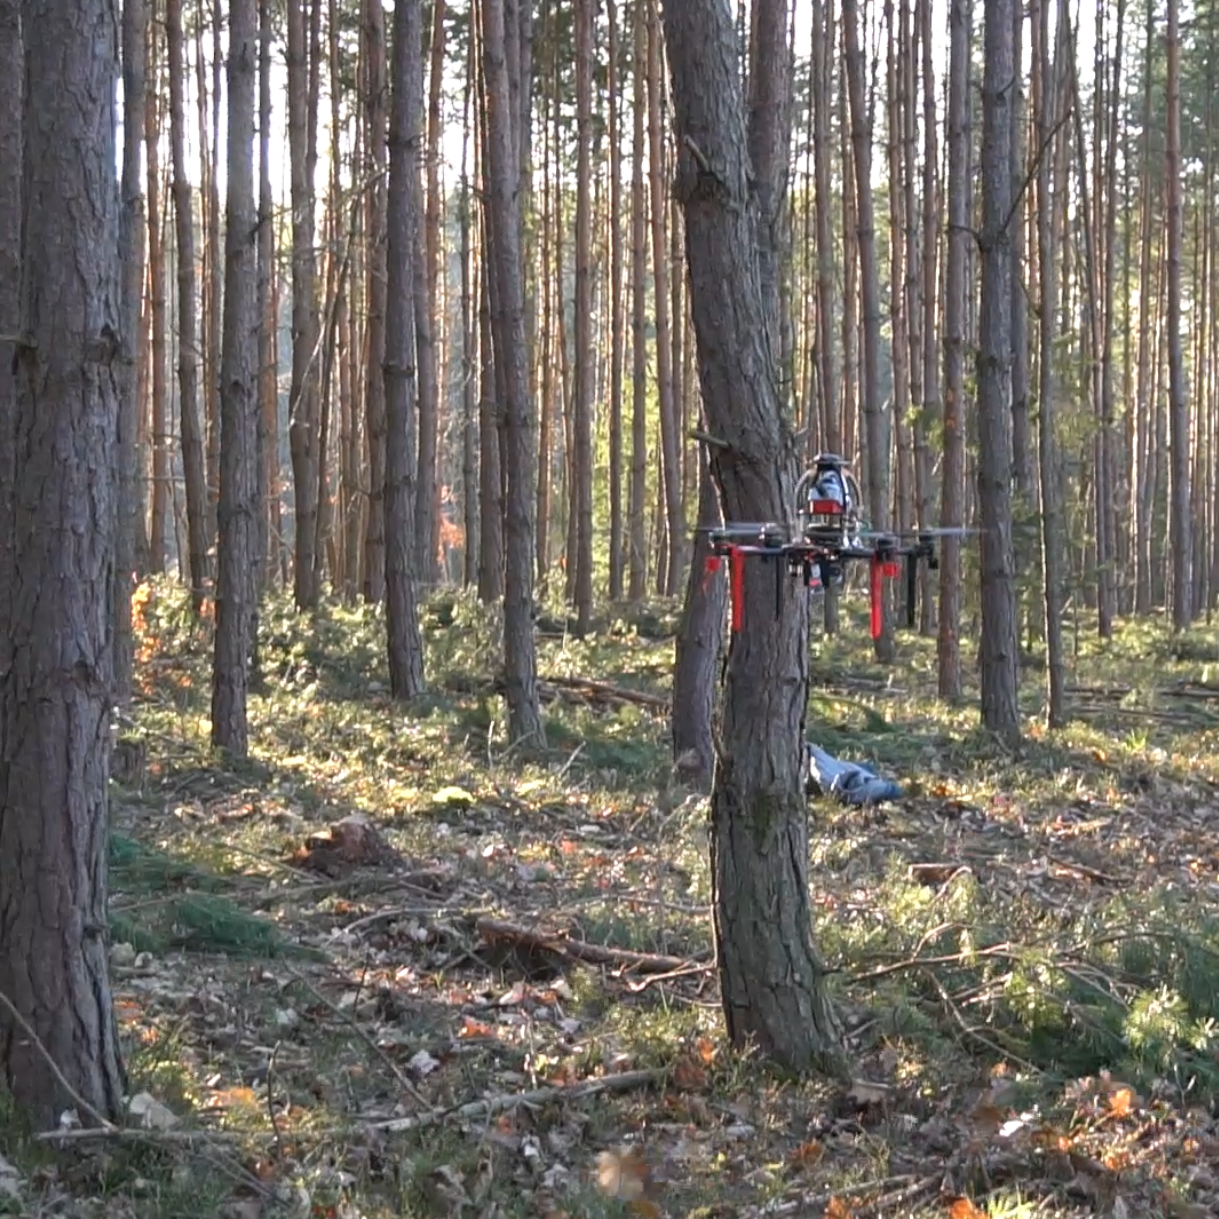
\includegraphics[width=0.48\textwidth]{./fig/photos/pic1.png}
                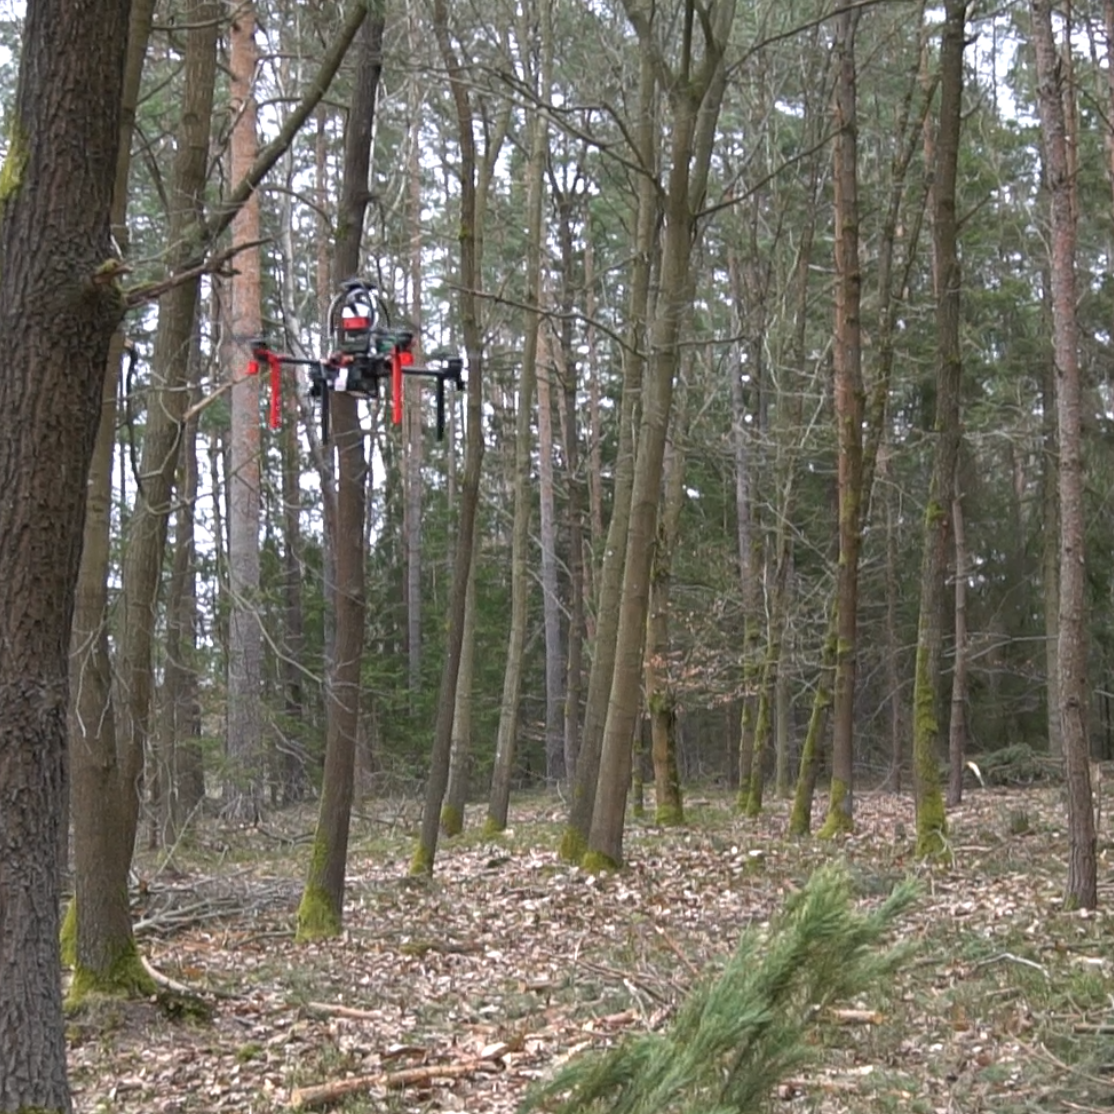
\includegraphics[width=0.48\textwidth]{./fig/photos/pic2.png}
                \caption{
                    The \ac{UAV} navigating in a forest during an experiment. 
                }
                \label{fig:real_wrld_pics}
            \end{figure}

            \begin{table}[H]
                \centering
                \caption{Parameters Used in Experiments}
                \begin{tabular}{|c|c|c|}
                    \hline
                    Parameter & Values Conservative & Values Aggressive \\
                    \hline
                    $r_s$ [m] & 2.0 & 2.0 \\ \hline
                    Update rate [Hz] & 10 & 10 \\ \hline
                    $\delta_i$ [m] & 0.5 & 0.5  \\ \hline
                    $d_1 = d_3 = d_5$ [m] & 0.5 & 0.5  \\ \hline
                    $d_2 = d_4 = d_6$ [m] & 1.0 & 1.0 \\ \hline
                    $\gamma$ [°] & 20.0 & 20.0 \\ \hline
                    $\beta_i^D$ [ ] & 0.5 & 0.1 \\ \hline
                    $\eta$ [ ] & 0.8 & 0.8 \\ \hline
                \end{tabular}
                \label{tab:rbl_forest_conservative_flight}
            \end{table}

            \begin{table}[H]
                \centering
                \renewcommand{\arraystretch}{1.2}
                \begin{tabular}{|c|c|c|c|c|}
                \hline
                                    & \( L \ [\mathrm{m}] \) & \( t \ [\mathrm{s}] \) &  \( v \ [\mathrm{m/s}] \)     \\ \hline
                Conservative Flight & 53.84                   & 116.40                  &  0.46                          \\ \hline
                Aggressive Flight    & 35.56                   &  51.64                  &  0.69                          \\ \hline
                \end{tabular}
            \end{table}

            \begin{figure}[htbp]
                \centering
                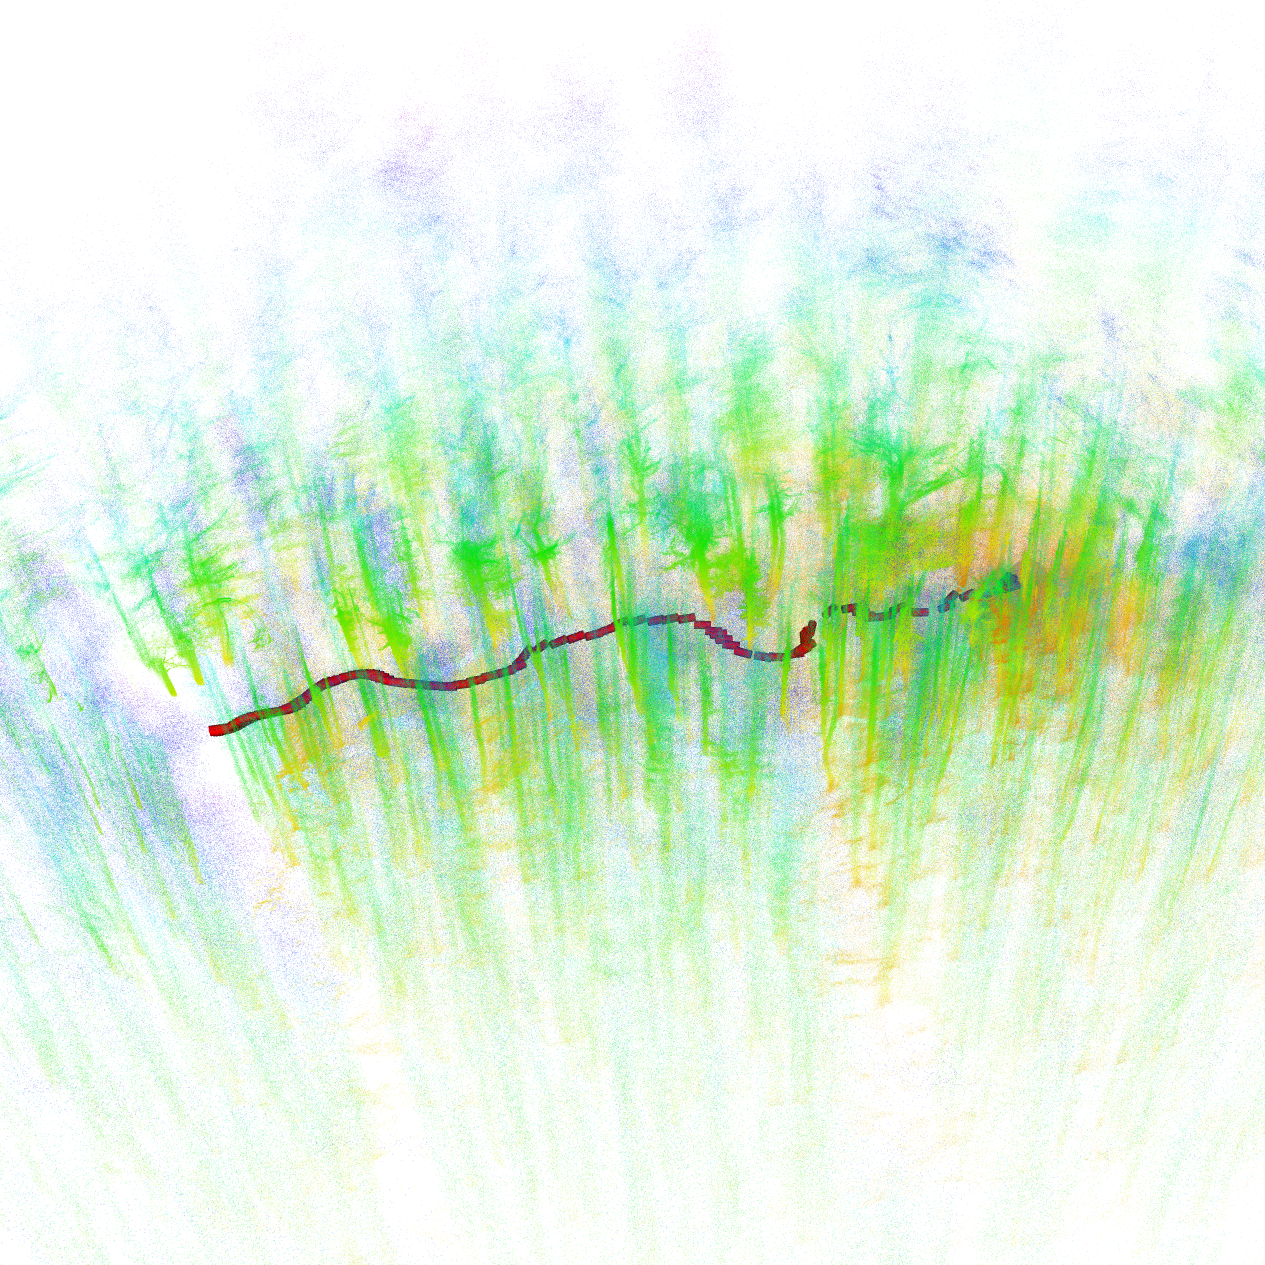
\includegraphics[width=0.48\textwidth]{./fig/rviz/flight_484.png}
                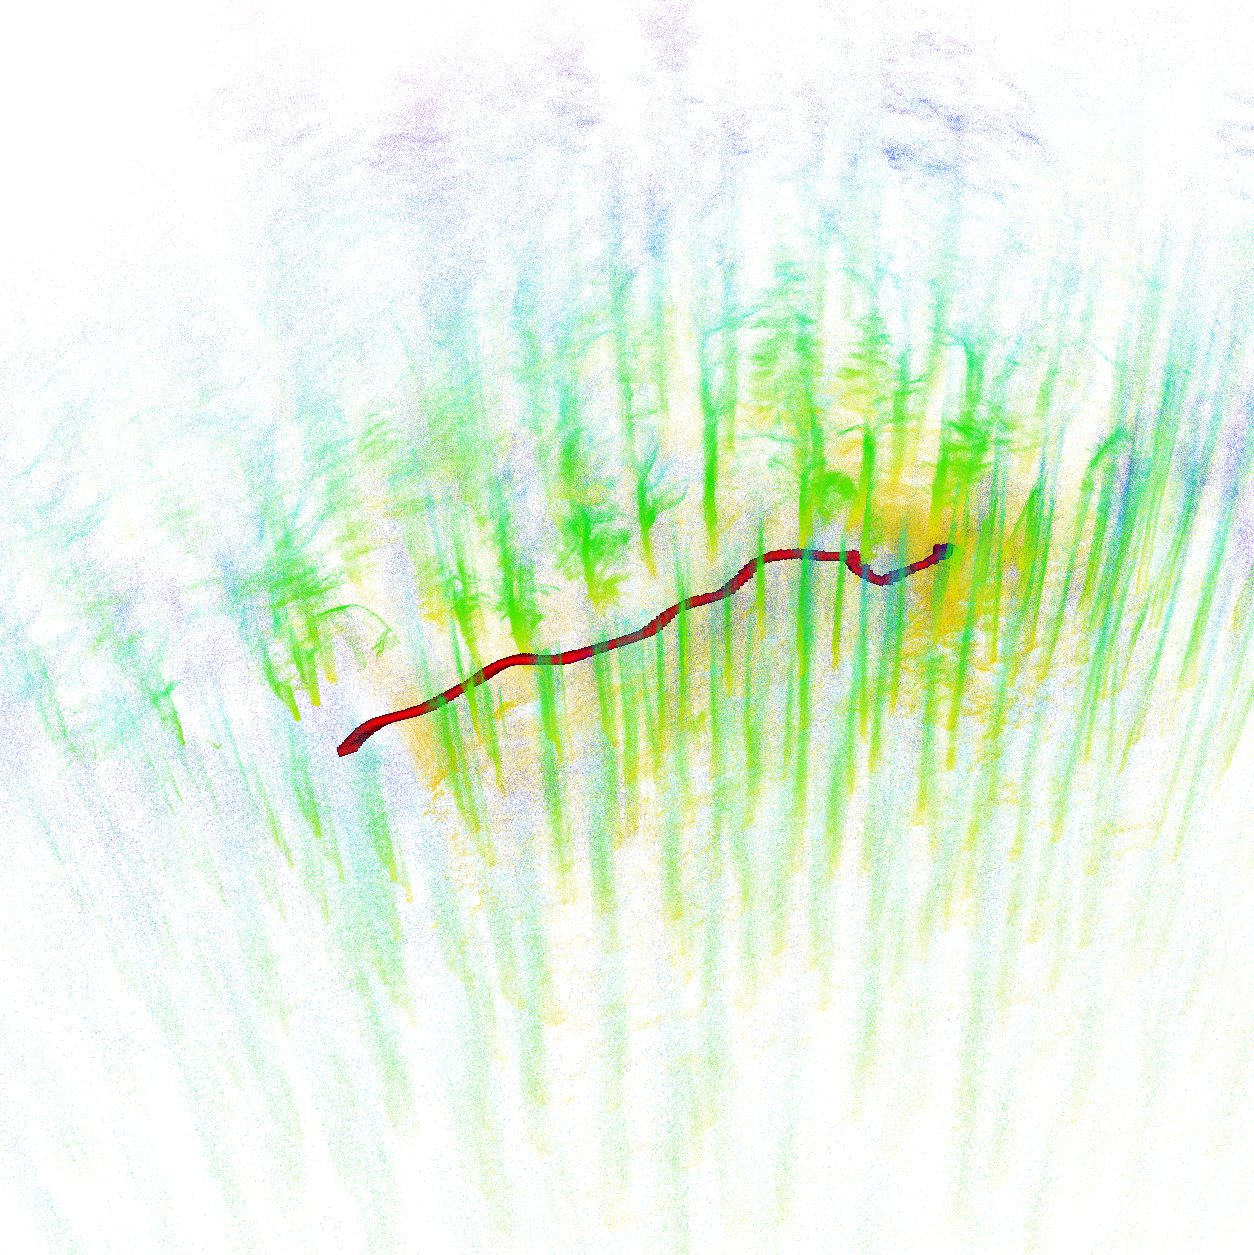
\includegraphics[width=0.48\textwidth]{./fig/rviz/flight_486.png}
                \caption{
                    \ac{UAV} flight trajectories through the forest test environment under different navigation settings. Left: Conservative parameter settings. Right: Aggressive parameter settings.
                }
                \label{fig:rbl_forest_conservative_flight_path}
            \end{figure}

        \subsection{Comparative Analysis}
            The real-world flight experiments conducted in the forest environment successfully validated the navigation capabilities of the proposed setup.
            The \ac{UAV} generally performed as expected based on simulation results, demonstrating its ability to navigate autonomously between points A and B while avoiding static obstacles.

            \subsection{Performance and Limitations}
                A primary limitation observed during real-world testing originated from the environmental mapping component, specifically the Bonxai mapping package used.
                While effective for static elements, the system occasionally struggled with dynamic obstacles, such as moving leaves.
                These obstacles were sometimes included in the voxel grid map and, due to the map's update policy (configured conservatively for safety), were not always removed immediately even when no longer present. 
                This could lead to situations where the \ac{UAV} perceived itself as blocked (as shown in the failure case video \cite{flight_fail}), requiring the safety pilot to land. 
                Addressing this mapping behavior is crucial for future testing.

            \subsection{Comparison with 2D Baseline}
                % Direct comparison with other state-of-the-art 3D navigation methods is challenging due to the specific nature of the RBL-based approach. 
                A meaningful comparison can be made with the original 2D RBL implementation \cite{rbl_paper}. 
                The key differences lie in the sensing and dimensionality:
                \begin{itemize}
                    \item The 2D version relied on a 2D \ac{LiDAR} for planar obstacle detection and a separate optical distance measurement sensor to maintain a constant flight altitude. 
                    Remapping obstacles in 2D is often simpler.
                    \item The 3D implementation utilizes a 3D \ac{LiDAR} for perception in three dimensions and must actively manage altitude based on the perceived environment, treating the ground itself as an obstacle.
                \end{itemize}
                A notable behavior observed in the 3D tests was the \ac{UAV}'s tendency to initially increase altitude after takeoff, effectively moving away from the ground obstacle, before potentially descending again as it got closer to the goal. 
                This behavior highlights the algorithm's capability to manage its vertical position based on the 3D environment.
                Regarding computational efficiency, while the 3D \ac{RBL} algorithm inherently involves greater complexity than its 2D counterpart (needing more points for 3D cell representation and more computational power for their partitioning), it nonetheless demonstrated manageable efficiency throughout the simulations and real-world flights.
                Illustrative examples of successful flights showcasing different parameter settings (\href{https://www.youtube.com/watch?v=DFt222gnA_w&ab_channel=MichalKamler}{aggressive} vs. \href{https://www.youtube.com/watch?v=AJPk0yVCPUo&ab_channel=MichalKamler}{conservative}) are provided in \cite{aggressive_flight} and \cite{conservative_flight}.

            \subsection{Future Work}
                The mapping limitations highlight key areas for future work. Potential solutions include:
                \begin{itemize}
                    \item \textbf{Dynamic Obstacle Handling: }\\
                    Implementing techniques to segment and filter out dynamic objects from the map representation such as \cite{TRLO_good_mapping}.
                    \item \textbf{Reactive Navigation: }\\
                    Exploring strategies that rely more on direct sensor input for immediate obstacle avoidance, removing dependence on the map, though this introduces challenges in perceiving areas outside the current sensor view (e.g. behind the UAV).
                    \item \textbf{Map-Based Strategic Replanning:} \\
                    Future work could include developing a higher-level path replanner that leverages the collected map to navigate agents around crowded areas, thereby supplementing the \ac{RBL} algorithm's local collision avoidance and enhancing overall efficiency.
                    \item \textbf{Map Update Logic: }\\
                    Investigating alternative mapping packages or implementing mechanisms like voxel decay instead of mapping (where unoccupied voxels gradually fade if not persistently observed) into the existing framework. 
                    While probabilistic mapping should ideally handle this, the developmental stage of the Bonxai package currently limits this capability.
                \end{itemize}
                Resolving these mapping challenges, particularly the robust handling of dynamic elements, is a prerequisite for advancing to more complex multi-agent experiments utilizing only onboard lidar sensing.
    
    \section{Conclusion}
    \label{sec:conclusion_lidar}
        This chapter detailed the implementation and real-world validation of the \ac{RBL} algorithm, adapted for autonomous \ac{UAV} navigation within a cluttered, \ac{GNSS}-denied forest environment using onboard 3D \ac{LiDAR} sensing. 
        The primary objective was to implement \ac{RBL} principles with real-time perception, state estimation (\ac{Point-LIO}), and mapping (Bonxai) to achieve reliable point-to-point navigation.

        Key technical contributions included adapting the \ac{RBL} algorithm's cell partitioning to directly utilize voxelized map data created from processed \ac{LiDAR} point clouds. 
        Modifications were also introduced to effectively handle the practical limitations of a single \ac{LiDAR} sensor with a restricted vertical field of view, ensuring safe convergence by constraining movement based on the actively sensed area while still leveraging map information. 
        An alternative approach using surface reconstruction via mesh generation was investigated but considered unsuitable due to computational complexity on the \ac{UAV} onboard computer.

        The proposed solution's effectiveness was demonstrated through both simulation and real-world experiments conducted in a forest. 
        The \ac{UAV} successfully navigated between designated start and goal points, avoiding static obstacles like trees and adapting its altitude based on the \ac{LiDAR}'s perception. 

        Despite the overall success, the experiments identified a key limitation related to the Bonxai mapping package's handling of dynamic environmental elements, such as moving leaves, which occasionally led to navigation deadlocks. 
        This emphasizes the importance of robust mapping with dynamic obstacles.

        In conclusion, this chapter successfully demonstrated the practical application and feasibility of using a 3D \ac{RBL} algorithm integrated with \ac{LiDAR} sensing for autonomous \ac{UAV} navigation in a challenging forest setting. 
        This capability can be observed in these videos \cite{aggressive_flight}, \cite{conservative_flight}.



